\chapter{Cinemática del aerogenerador}
\label{ch:cinematica}
\section{Cuerpo material, configuración y movimiento}
\subsection{Cuerpo material y descripción del movimiento}
Un cuerpo material $\mathcal B$ es un conjunto de partículas cuya identidad se conserva durante el movimiento. Una partícula no se define por la posición que ocupa en un instante: puede cambiar de posición sin dejar de ser la misma partícula. La torre, cada pala y cada pieza rígida se consideran cuerpos distintos. El sistema completo es una colección de cuerpos con interfaces y vínculos; las partículas de dos cuerpos conectados no se identifican entre sí por compartir una posición en la unión.

Una configuración asigna a cada partícula un punto del espacio euclídeo. La configuración de referencia se denota $\mathcal B_0$ y permite etiquetar una partícula por su posición $\vct X$. La configuración actual, $\mathcal B_t$, es el lugar que ocupa el cuerpo en el instante $t$ y usa posiciones $\vct x$. Esta distinción material--espacial, habitual en mecánica del continuo \cite{holzapfel}, permite describir el movimiento como
\begin{equation}
 \vct x=\vct\chi(\vct X,t),\qquad
 \vct\chi(\cdot,t):\mathcal B_0\longrightarrow\mathcal B_t.
 \label{eq:chi}
\end{equation}
La letra $\vct X$ identifica una posición de referencia, no un sistema de coordenadas. La misma $\vct X$ aparece para una partícula a lo largo de toda su trayectoria. En cambio, $\vct x$ depende del tiempo. Se exige localmente que el movimiento sea diferenciable e invertible y que conserve la orientación del material.

\subsection{Configuración de referencia y ausencia de tensiones}
La elección de $\mathcal B_0$ es parte de la descripción. Puede coincidir con una geometría de fabricación, una geometría descargada o una geometría precargada conocida. No es automáticamente una configuración sin tensiones. Si se adopta una geometría descargada y una ley constitutiva que asigna tensión nula a deformación nula, ambas propiedades coinciden por hipótesis, no por definición.

Para esta tesis, se toma como referencia geométrica la torre y las palas con su forma nominal de montaje, en un azimut seleccionado. La precurvatura y la pretorsión, si se incluyen, pertenecen a esa geometría inicial y no deben producir tensiones elásticas por sí solas. La deformación debida a cargas de operación se calcula respecto a ella. Esta elección debe mantenerse al interpretar las propiedades geométricas, las longitudes y las orientaciones de sección.

La figura~\ref{fig:configs} representa esta correspondencia material y permite leer el desplazamiento como la diferencia de dos posiciones medidas desde el mismo origen.

\begin{figure}[htbp]
\centering
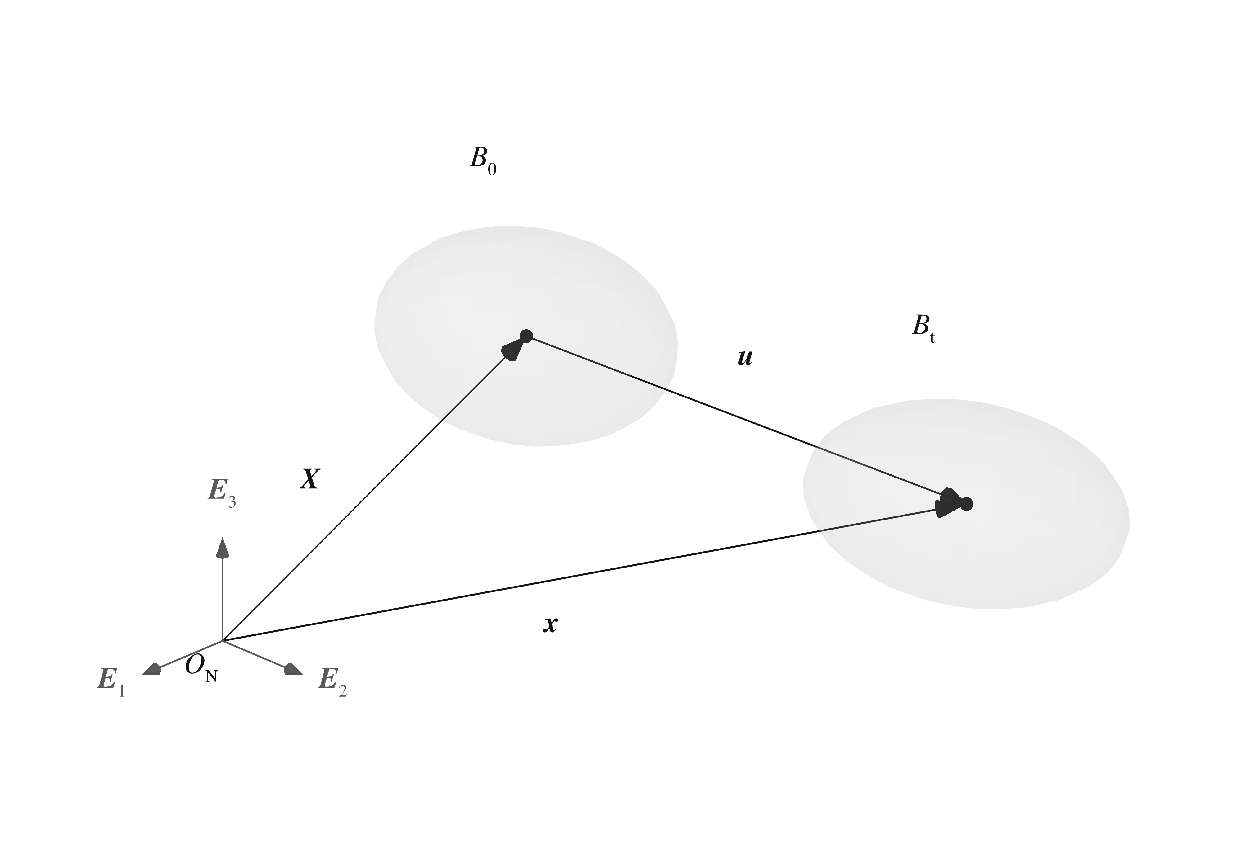
\includegraphics[width=.96\linewidth,height=.40\textheight,keepaspectratio]{figures/tecplot/concept_configs.pdf}
\caption[Configuraciones de referencia y actual]{Una misma partícula en las configuraciones de referencia y actual. Los vectores $\vct X$ y $\vct x$ se miden desde $O_N$ y su diferencia define $\vct u$. Las envolventes transparentes identifican el cuerpo material; la geometría es ilustrativa.}\label{fig:configs}
\end{figure}

\subsection{Desplazamiento y movimiento de cuerpo rígido}
En un origen y una base comunes, el desplazamiento material es
\begin{equation}
 \vct u(\vct X,t)=\vct\chi(\vct X,t)-\vct X.
\end{equation}
Incluye traslaciones y rotaciones rígidas. Por ejemplo, $\vct\chi=\vct c(t)+\ten Q(t)\vct X$ describe un movimiento rígido si $\ten Q^\tr\ten Q=\Id$ y $\det\ten Q=1$. Entonces $\vct u=\vct c+(\ten Q-\Id)\vct X$ puede ser grande, pero las distancias entre partículas no cambian. Por ello no se usa el tamaño del desplazamiento inercial como medida directa de la deformación de una pala en giro.

\section{Herramientas tensoriales y convención de componentes}
\subsection{Vectores, tensores y productos}
Un vector geométrico se escribe $\vct a$ y un tensor de segundo orden $\ten A$. En una base ortonormal dextrógira $\{\vct e_i\}$,
\begin{equation}
 \vct a=a_i\vct e_i,\qquad \ten A=A_{ij}\vct e_i\otimes\vct e_j.
\end{equation}
Se suman los índices repetidos de 1 a 3. El producto diádico se define por $(\vct a\otimes\vct b)\vct c=\vct a(\vct b\cdot\vct c)$. El producto escalar de tensores es $\ten A:\ten B=\operatorname{tr}(\ten A^\tr\ten B)$. La identidad satisface $\Id\vct a=\vct a$.

Para una terna de componentes $\vct a=(a_1,a_2,a_3)^\tr$, se define
\begin{equation}
 \sk a=\begin{bmatrix}0&-a_3&a_2\\a_3&0&-a_1\\-a_2&a_1&0\end{bmatrix},
 \qquad \sk a\vct b=\vct a\times\vct b,
 \qquad \sk a^\tr=-\sk a.
 \label{eq:skew}
\end{equation}
El símbolo $[\cdot]_\times$ es una aplicación que asocia a un vector una matriz antisimétrica. Su inversa sobre matrices antisimétricas se denota $\ax$. No es una fuerza ni una rigidez; es una herramienta para representar productos vectoriales.

\subsection{Sistema de referencia y cambio de componentes}
Un sistema de referencia $\mathcal F_A$ consta de un origen $O_A$ y una base ortonormal $\{\vct e_i^A\}$. Para expresar un vector en esa base se escribe ${}^A\vct a$. La matriz ${}^A Q_B$ contiene en sus columnas los ejes de $B$ expresados en $A$:
\begin{equation}
 ({}^A Q_B)_{ij}=\vct e_i^A\cdot\vct e_j^B,
 \quad {}^A\vct a={}^A Q_B\,{}^B\vct a,
 \quad {}^B Q_A=({}^A Q_B)^\tr.
 \label{eq:componentes}
\end{equation}
La composición respeta el orden de los sistemas de referencia: ${}^A Q_C={}^A Q_B{}^B Q_C$. Para un tensor físico,
\begin{equation}
 [\ten A]^A={}^A Q_B[\ten A]^B({}^A Q_B)^\tr.
\end{equation}
Cambiar componentes no cambia el vector físico. En contraste, aplicar una rotación física a un cuerpo modifica sus directores y posiciones. Aunque ambas operaciones se representen por matrices ortogonales, su interpretación es distinta.

La figura~\ref{fig:cambio-componentes} permite leer geométricamente la ecuación~\eqref{eq:componentes}. Las proyecciones sobre cada par de ejes producen números diferentes, pero todas representan el mismo vector. La rotación de la base no debe confundirse con el desplazamiento de una partícula.
\begin{figure}[htbp]
\centering
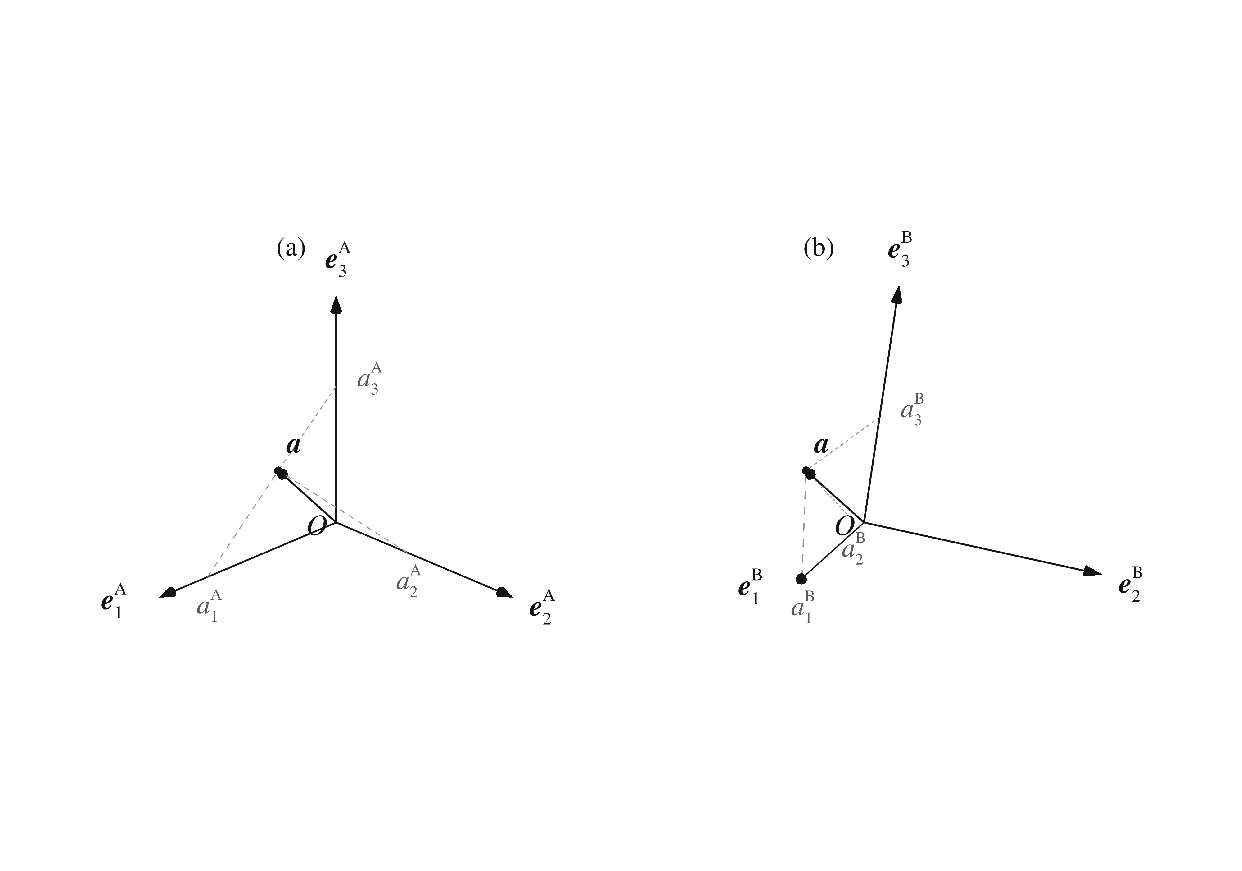
\includegraphics[width=.96\linewidth,height=.40\textheight,keepaspectratio]{figures/tecplot/concept_cambio-componentes.pdf}
\caption[Componentes de un vector en dos bases]{Un mismo vector espacial $\vct a$ expresado en las bases $A$ y $B$, representadas por separado en (a) y (b). Las líneas auxiliares relacionan la punta con sus proyecciones sobre cada eje. Cambian las componentes $a_i^A$ y $a_i^B$, mientras se conserva el vector geométrico.}\label{fig:cambio-componentes}
\end{figure}

Para una posición debe incluirse también la traslación del origen:
\begin{equation}
 {}^A\vct x={}^A\vct c_B+{}^A Q_B{}^B\vct y,
 \label{eq:affine}
\end{equation}
donde $\vct c_B$ une $O_A$ con $O_B$ y $\vct y$ une $O_B$ con el punto. No se traslada un vector libre, como una velocidad relativa o una fuerza, del mismo modo que una posición. La velocidad absoluta requiere además diferenciar los movimientos del origen y de la base.

Si también cambia el origen, la transformación de componentes se combina con una traslación, como muestra la figura~\ref{fig:frames}.

\begin{figure}[htbp]
\centering
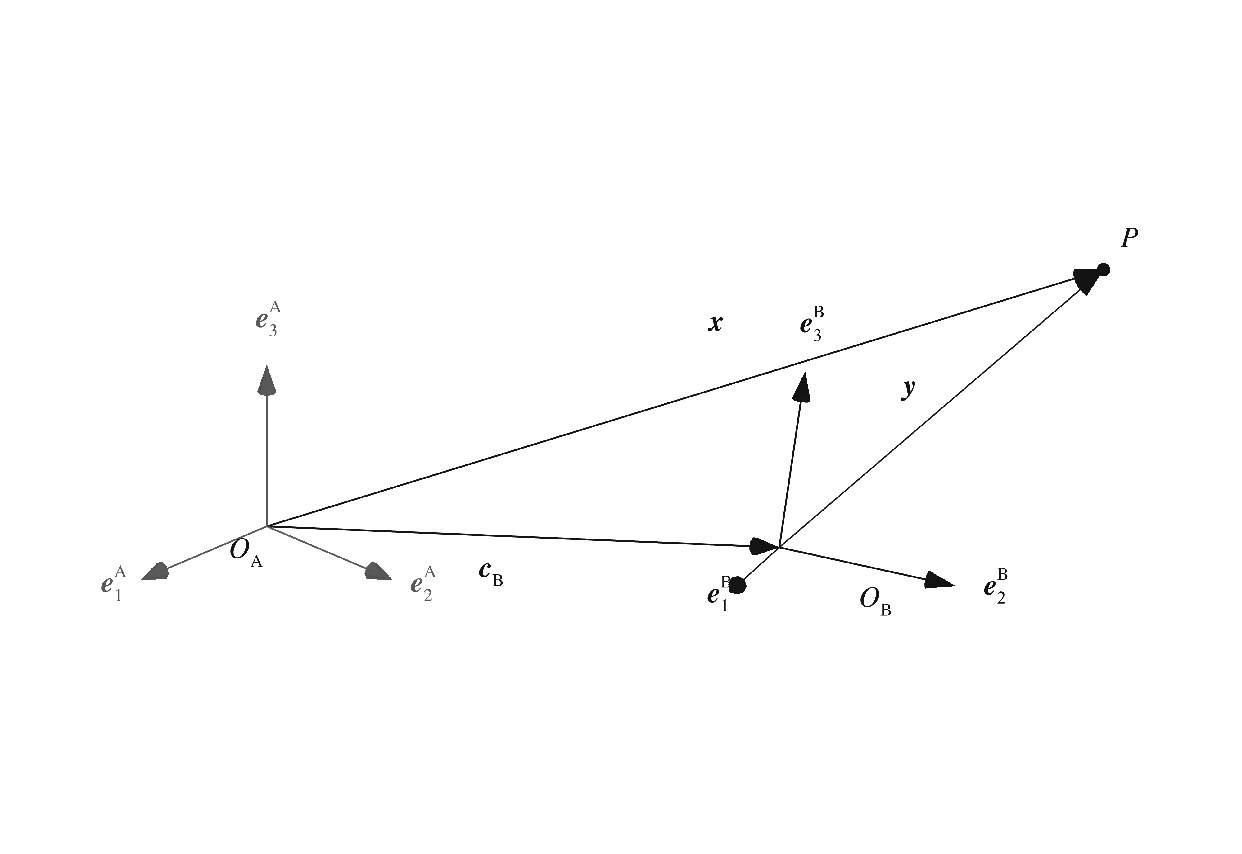
\includegraphics[width=.96\linewidth,height=.40\textheight,keepaspectratio]{figures/tecplot/concept_frames.pdf}
\caption[Cambio de origen y de base]{Cambio de origen y de base en el espacio. Los tres ejes de cada triedro permiten distinguir orientación y posición. Se cumple $\vct x=\vct c_B+\vct y$ como identidad vectorial; en componentes de $A$, ${}^A\vct x={}^A\vct c_B+{}^AQ_B{}^B\vct y$.}\label{fig:frames}
\end{figure}

\subsection{Matrices de rotación y orientación relativa}
La orientación de dos bases puede construirse mediante rotaciones elementales. Se adopta el sentido positivo de la regla de la mano derecha: el pulgar señala el eje positivo y el cierre de los dedos indica el sentido de giro. Las matrices que representan rotaciones de un vector alrededor de los ejes 1, 2 y 3 de una base ortonormal son
\begin{align}
 R_1(\alpha)&=
 \begin{bmatrix}1&0&0\\0&\cos\alpha&-\sin\alpha\\0&\sin\alpha&\cos\alpha\end{bmatrix},
 \label{eq:R1}\\
 R_2(\beta)&=
 \begin{bmatrix}\cos\beta&0&\sin\beta\\0&1&0\\-\sin\beta&0&\cos\beta\end{bmatrix},
 \label{eq:R2}\\
 R_3(\gamma)&=
 \begin{bmatrix}\cos\gamma&-\sin\gamma&0\\\sin\gamma&\cos\gamma&0\\0&0&1\end{bmatrix}.
 \label{eq:R3}
\end{align}
Cada matriz deja inalterada la componente sobre el eje de giro y transforma las dos componentes del plano perpendicular. Por ejemplo, $R_1(\alpha)\vct e_2=\cos\alpha\,\vct e_2+\sin\alpha\,\vct e_3$. Sus columnas son las imágenes de los tres vectores de la base inicial. La ortogonalidad se expresa por $R_i^\tr R_i=\Id$ y el determinante positivo conserva la orientación dextrógira.

La figura~\ref{fig:rotaciones-elementales} presenta cada rotación elemental mediante el triedro completo y el arco en el plano perpendicular a su eje. Al observar desde el semieje positivo hacia el origen, el giro positivo se ve antihorario. Las etiquetas de los ejes, y no su posición en la página, determinan qué matriz corresponde a cada panel.

\begin{figure}[htbp]
\centering
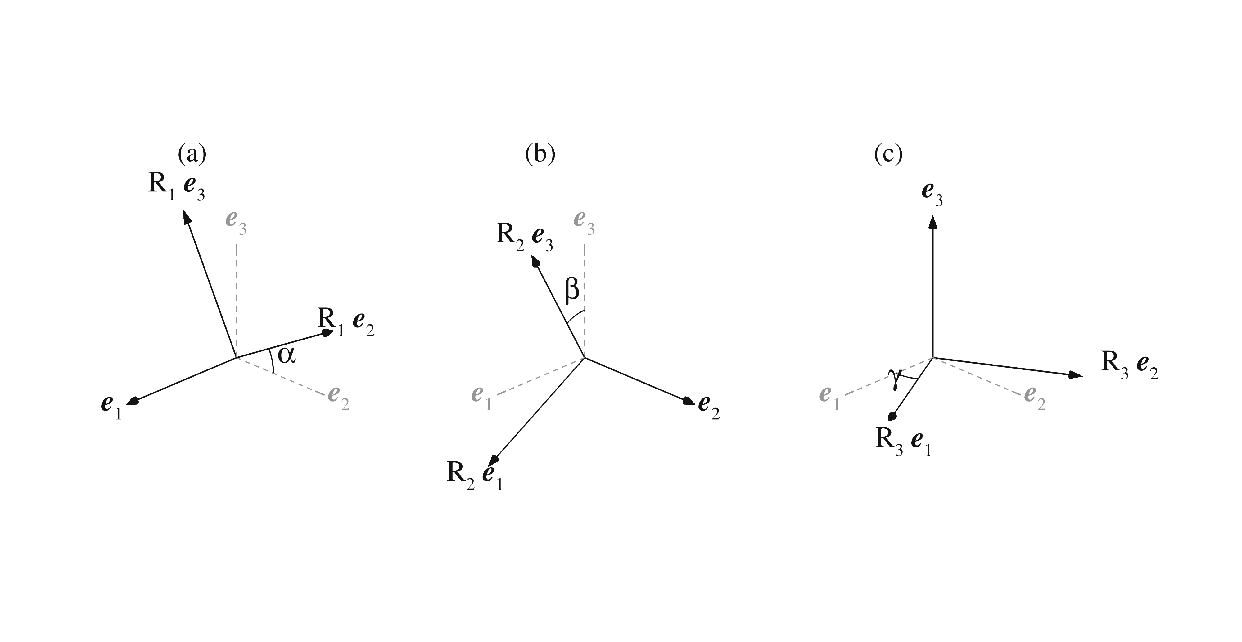
\includegraphics[width=.96\linewidth,height=.40\textheight,keepaspectratio]{figures/tecplot/concept_rotaciones-elementales.pdf}
\caption[Rotaciones elementales]{Rotaciones elementales en tres dimensiones: (a) $R_1(\alpha)$, (b) $R_2(\beta)$ y (c) $R_3(\gamma)$. Las direcciones iniciales se trazan discontinuas en gris y sus imágenes continuas en negro. El eje de giro permanece inalterado; los arcos siguen la regla de la mano derecha. Los ángulos son ilustrativos.}\label{fig:rotaciones-elementales}
\end{figure}

Si una base se obtiene girando sus propios ejes, la orientación final se construye multiplicando a la derecha la matriz de cada rotación sucesiva. Una secuencia de giros $\alpha,\beta,\gamma$ alrededor de los ejes móviles 1, 2 y 3 se representa por
\begin{equation}
 {}^A Q_B=R_1(\alpha)R_2(\beta)R_3(\gamma).
 \label{eq:cardan}
\end{equation}
Estos tres parámetros constituyen una secuencia de ángulos de Cardan. El orden forma parte de la definición: en general $R_1R_2\ne R_2R_1$. Por otra parte, expresar en $B$ las componentes de un vector conocido en $A$ requiere la matriz transpuesta $({}^AQ_B)^\tr$. Así se distinguen una rotación física, que cambia la orientación del cuerpo, y un cambio de base, que representa el mismo vector con otras componentes.

El conjunto de las matrices de rotación propias se denota
\begin{equation}
 \SO=\{Q\in\R^{3\times3}:Q^\tr Q=\Id,\ \det Q=1\}.
\end{equation}
Esta notación reúne las dos condiciones geométricas que ya se han establecido: conservación de longitudes y ángulos, y conservación de la orientación de la base.

La figura~\ref{fig:rotacion-bases} distingue la rotación de los ejes de la representación de un mismo vector en las dos bases.

\begin{figure}[htbp]
\centering
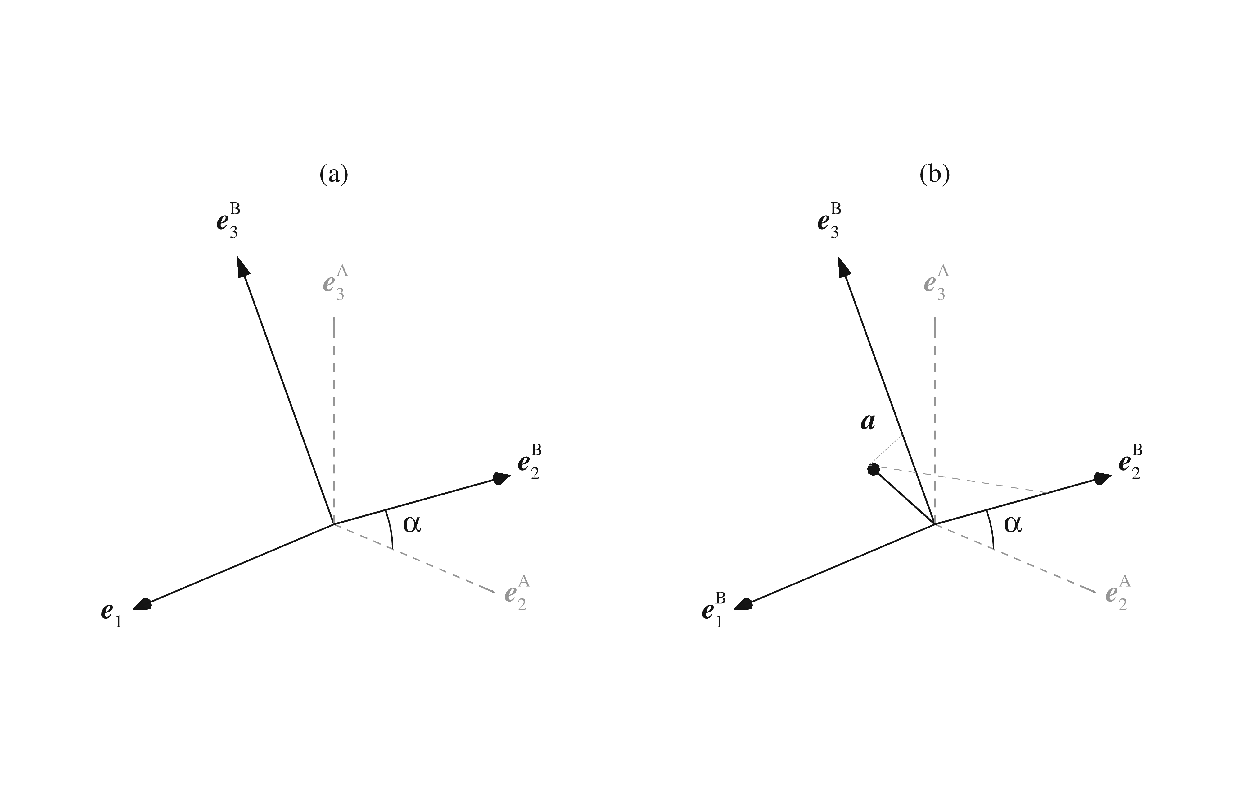
\includegraphics[width=.96\linewidth,height=.40\textheight,keepaspectratio]{figures/tecplot/concept_rotacion-bases.pdf}
\caption[Rotación de ejes y cambio de componentes]{(a) Rotación de un triedro alrededor de su eje 1. (b) Representación de un vector fijo en la base inicial y la girada. Las líneas discontinuas identifican la orientación inicial y las continuas la girada; las proyecciones se leen respecto de sus ejes respectivos. La matriz de orientación y su transpuesta tienen funciones distintas.}\label{fig:rotacion-bases}
\end{figure}

\subsection{Derivación de la velocidad angular}
La derivada de un vector de la base solidaria con un cuerpo rígido es perpendicular a ese vector. Además, la ortogonalidad entre ejes se conserva. Estas condiciones se reúnen en una única velocidad angular $\vct\omega_{B/A}$, relativa a $A$, que satisface
\begin{equation}
 \left(\frac{\dd\vct e_i^B}{\dd t}\right)_A
 =\vct\omega_{B/A}\times\vct e_i^B.
 \label{eq:derivada-ejes}
\end{equation}
El subíndice exterior indica el sistema de referencia desde el cual se deriva; el cociente $B/A$ identifica el movimiento relativo. Para $Q={}^AQ_B$, la ecuación anterior aplicada a sus tres columnas da
\begin{equation}
 \dot Q=[{}^A\vct\omega_{B/A}]_\times Q
       =Q[{}^B\vct\omega_{B/A}]_\times,\qquad
 [ {}^A\vct\omega_{B/A}]_\times=\dot Q Q^\tr.
 \label{eq:Qdot}
\end{equation}
La antisimetría también se deduce diferenciando $QQ^\tr=\Id$. Si se utiliza la transformación inversa $C=Q^\tr$, su derivada es
\begin{equation}
 \dot C=-[{}^B\vct\omega_{B/A}]_\times C.
 \label{eq:Cdot}
\end{equation}
El signo diferente corresponde a la transformación inversa y a las componentes en el sistema solidario con el cuerpo de la velocidad angular. Las dos ecuaciones describen el mismo movimiento.

Para la secuencia de \eqref{eq:cardan}, cada giro aporta una velocidad angular sobre su eje instantáneo:
\begin{equation}
 \vct\omega_{B/A}
 =\dot\alpha\,\vct e_1^A
  +\dot\beta\,\vct e_2^{(1)}
  +\dot\gamma\,\vct e_3^B.
\end{equation}
La base intermedia $(1)$ se obtiene después del primer giro. Expresando los tres ejes en la base final $B$ se obtiene
\begin{equation}
 {}^B\vct\omega_{B/A}=
 \begin{bmatrix}
 \cos\beta\cos\gamma&\sin\gamma&0\\
 -\cos\beta\sin\gamma&\cos\gamma&0\\
 \sin\beta&0&1
 \end{bmatrix}
 \begin{bmatrix}\dot\alpha\\\dot\beta\\\dot\gamma\end{bmatrix}.
 \label{eq:cardan-velocidad}
\end{equation}
Por tanto, las derivadas de los ángulos no son, en general, las componentes de la velocidad angular. La matriz de esta relación tiene determinante $\cos\beta$ y pierde invertibilidad para $\beta=\pm\pi/2$. Se trata de una singularidad de las coordenadas angulares, no de una singularidad del movimiento físico. Las matrices de orientación permiten describir el giro nominal sin recurrir a la inversión de esta relación; las perturbaciones pequeñas se parametrizan más adelante mediante un vector de rotación.

La figura~\ref{fig:derivada-director} interpreta la ecuación~\eqref{eq:derivada-ejes} mediante dos orientaciones próximas de un mismo director. El cambio del director es tangente a su esfera unitaria en el límite temporal. La velocidad angular no mide el cambio de longitud del eje, sino la rapidez y la dirección de su cambio de orientación.

\begin{figure}[htbp]
\centering
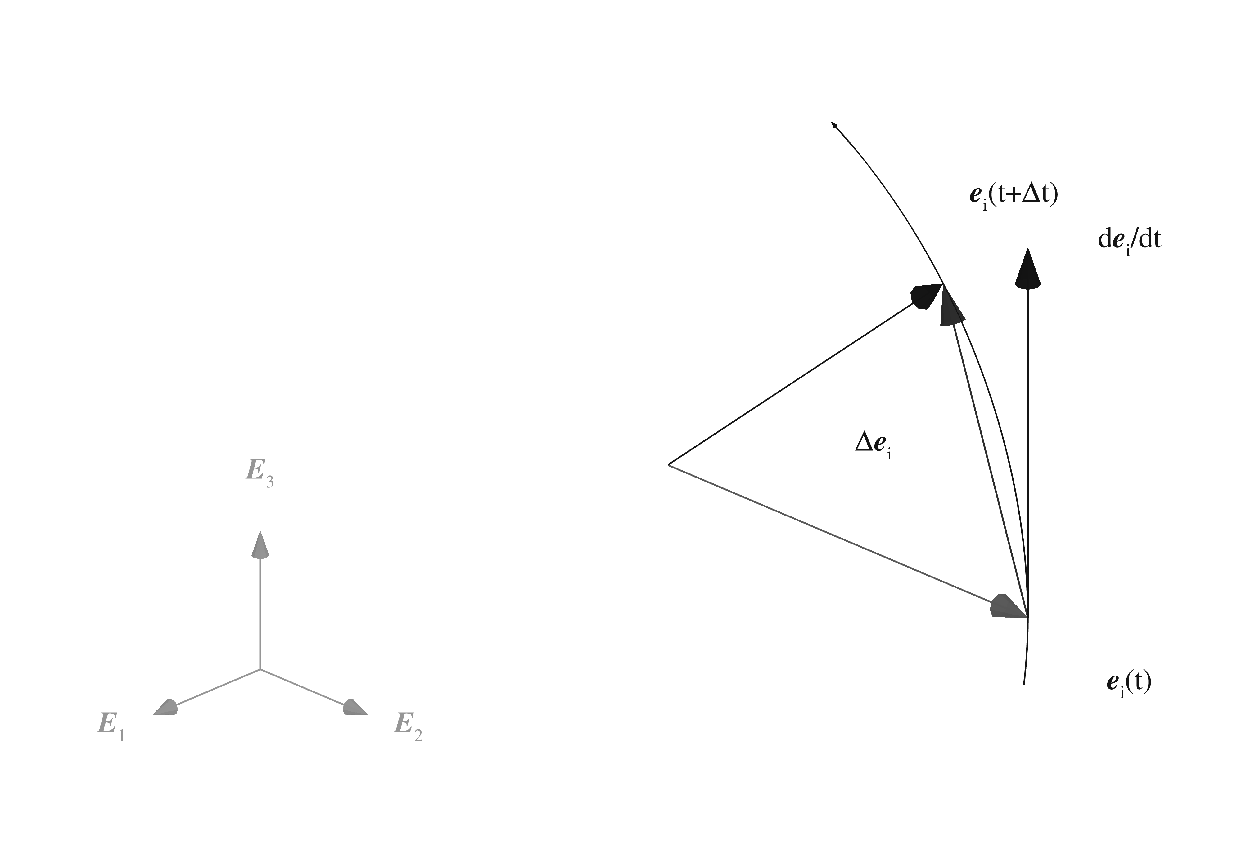
\includegraphics[width=.96\linewidth,height=.40\textheight,keepaspectratio]{figures/tecplot/concept_derivada-director.pdf}
\caption[Derivada temporal de un director]{Evolución espacial de un director de longitud constante. La cuerda une $\vct e_i(t)$ y $\vct e_i(t+\Delta t)$ y representa $\Delta\vct e_i$; la derivada en $t$ es tangente a la trayectoria circular y perpendicular al director. Las longitudes se amplían para mostrar su relación geométrica.}\label{fig:derivada-director}
\end{figure}

\subsection{Derivada de un vector en una base móvil}
Sea $\vct a=a_i^B(t)\vct e_i^B(t)$. Al aplicar la regla de derivación del producto,
\begin{equation}
 \left(\frac{\dd\vct a}{\dd t}\right)_A
 =\dot a_i^B\vct e_i^B+
   a_i^B\left(\frac{\dd\vct e_i^B}{\dd t}\right)_A
 =\left(\frac{\dd\vct a}{\dd t}\right)_B+
   \vct\omega_{B/A}\times\vct a.
 \label{eq:teorema-transporte}
\end{equation}
Esta identidad es el teorema de transporte de la derivada de un vector. Su primer término representa el cambio de las componentes medidas en $B$; el segundo representa el cambio de la base. Para un vector fijo en el cuerpo, el primer término es nulo, aunque la derivada observada desde $A$ no lo sea. Para una pala flexible, en cambio, sus vectores de posición relativos varían también por deformación y ambos términos intervienen.

La composición de orientaciones $ {}^NQ_P={}^NQ_H{}^HQ_P$, al ser derivada y multiplicada por su transpuesta, conduce a la composición de velocidades angulares
\begin{equation}
 {}^N\vct\omega_{P/N}
 ={}^N\vct\omega_{H/N}
  +{}^NQ_H\,{}^H\vct\omega_{P/H}.
 \label{eq:composicion-omega}
\end{equation}
Las velocidades angulares se suman como vectores una vez expresadas en una base común. Esta propiedad no implica que puedan sumarse del mismo modo los ángulos de rotaciones finitas.

\section{Medidas de deformación del continuo}
La derivada material del movimiento es el gradiente de deformación:
\begin{equation}
 \ten F=\Grad_{\!X}\vct\chi,
 \qquad \dd\vct x=\ten F\dd\vct X,
 \qquad J=\det\ten F>0.
\end{equation}
El tensor $\ten F$ transporta segmentos infinitesimales desde la configuración de referencia a la actual; no es simplemente una matriz de rotación. Es un tensor de dos puntos: su argumento pertenece al espacio tangente material y su imagen al espacial. En componentes, $F_{iA}=\partial x_i/\partial X_A$; el índice mayúsculo identifica el lado material, no una potencia. El escalar $J$ mide la razón local de volumen, $\dd V=J\dd V_0$. Para masa conservada, $\rho J=\rho_0$. El símbolo $J$ sin índice no se usa aquí para el tensor de inercia, que se escribe $\ten J_C$.

Al comparar longitudes se obtiene
\begin{align}
 \dd\vct x\cdot\dd\vct x&=\dd\vct X\cdot\ten C\dd\vct X,
 &\ten C&=\ten F^\tr\ten F,\\
 \ten E&=\tfrac12(\ten C-\Id),
 &\|\dd\vct x\|^2-\|\dd\vct X\|^2&=2\dd\vct X\cdot\ten E\dd\vct X.
\end{align}
Aquí $\ten E$ es la deformación de Green--Lagrange. Para un movimiento rígido $\ten F=\ten Q$, se tiene $\ten C=\Id$ y $\ten E=\ten0$. Esta comprobación distingue una descripción geométricamente consistente de una que interpreta el giro como deformación.

Si $\ten H=\Grad\vct u$, la identidad exacta es
\begin{equation}
 \ten E=\tfrac12(\ten H+\ten H^\tr+\ten H^\tr\ten H).
\end{equation}
Solo cuando el gradiente de desplazamiento es pequeño puede despreciarse el último término. En el rotor, el giro nominal grande debe separarse antes de aplicar esa aproximación. Linealizar directamente el desplazamiento total inercial a lo largo de una revolución generaría deformaciones ficticias.

La descomposición polar $\ten F=\ten R\ten U=\ten V\ten R$ separa una rotación de un estiramiento, con $\ten R\in\SO$ y $\ten U$, $\ten V$ simétricos positivos. No debe confundirse esa rotación polar del continuo con la rotación de un triedro de sección: en una viga con cortante, el director longitudinal no coincide necesariamente con la tangente a la línea media ni con la rotación polar local.

\subsection{Dos movimientos que permiten interpretar las medidas}
Para un bloque que gira rígidamente un ángulo $\alpha$ en el plano 1--2, $\ten F=R_3(\alpha)$ y $\ten E=0$. Sin embargo, si se aplicara la medida infinitesimal al desplazamiento total, se obtendría
\begin{equation}
 \sym\Grad\vct u=\sym(R_3(\alpha)-\Id)
 =\diag(\cos\alpha-1,\cos\alpha-1,0).
\end{equation}
Para un ángulo finito esta matriz no es cero: el resultado no revela una deformación física, sino el uso de una aproximación fuera de su dominio. Esto justifica separar el giro nominal del rotor antes de introducir una deformación lineal.

En cambio, el movimiento $x_1=X_1+kX_2$, $x_2=X_2$, $x_3=X_3$ es un cortante simple. Su gradiente y su medida de Green--Lagrange son
\begin{equation}
 F=\begin{bmatrix}1&k&0\\0&1&0\\0&0&1\end{bmatrix},\qquad
 E=\frac12\begin{bmatrix}0&k&0\\k&k^2&0\\0&0&0\end{bmatrix}.
\end{equation}
Se conserva el volumen porque $\det F=1$, pero cambian ángulos y longitudes. Una fibra inicialmente paralela al eje 2 adquiere longitud multiplicada por $\sqrt{1+k^2}$. A primer orden se retiene $E_{12}=k/2$ y se desprecia $k^2/2$; esa aproximación requiere $|k|\ll1$. Ni conservación de volumen ni gran desplazamiento bastan por sí solos para identificar la deformación.

La figura~\ref{fig:rotacion-deformacion} compara ambos movimientos mediante una cuadrícula material: la rotación conserva los ángulos entre sus líneas, mientras que el cortante los modifica.

\begin{figure}[htbp]
\centering
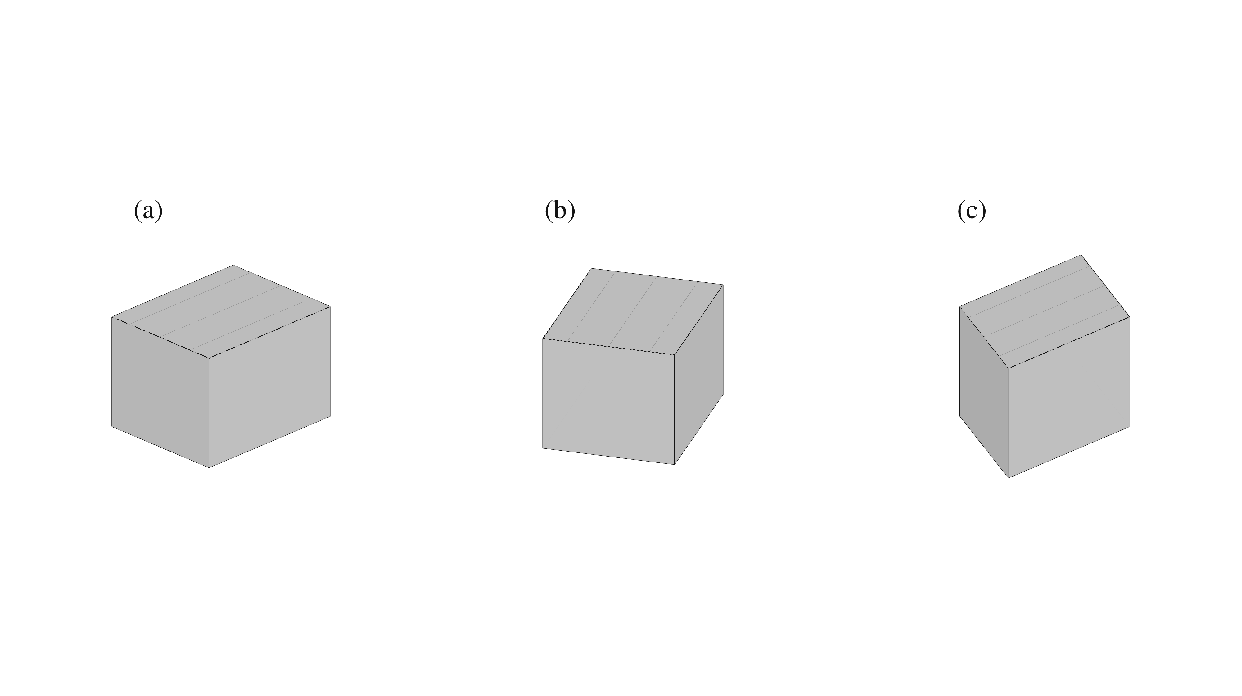
\includegraphics[width=.96\linewidth,height=.40\textheight,keepaspectratio]{figures/tecplot/concept_rotacion-deformacion.pdf}
\caption[Rotación rígida y deformación por cortante]{Una misma porción material en tres dimensiones: (a) referencia, (b) rotación rígida y (c) deformación por cortante. La cuadrícula identifica líneas materiales. La rotación conserva los ángulos y las longitudes; la deformación cambia la forma.}\label{fig:rotacion-deformacion}
\end{figure}

\section{Velocidad, aceleración y derivadas}
La velocidad y aceleración materiales se calculan manteniendo fija la etiqueta $\vct X$:
\begin{equation}
 \vct v(\vct X,t)=\left.\frac{\partial\vct\chi}{\partial t}\right|_X,
 \qquad \vct a(\vct X,t)=\left.\frac{\partial^2\vct\chi}{\partial t^2}\right|_X.
\end{equation}
Una representación espacial de la velocidad se obtiene sustituyendo $\vct X=\vct\chi^{-1}(\vct x,t)$. Para un campo espacial $\vct w(\vct x,t)$, la derivada siguiendo una partícula es
\begin{equation}
 \frac{D\vct w}{Dt}=\frac{\partial\vct w}{\partial t}+(\grad\vct w)\vct v.
\end{equation}
No se intercambia esa derivada con una derivada a posición espacial fija. El gradiente espacial de velocidad satisface $\ten l=\dot{\ten F}\ten F^{-1}$ y se separa en $\ten d=\sym\ten l$ y $\ten w=(\ten l-\ten l^\tr)/2$. El segundo es el tensor de giro local del continuo; el símbolo $\ten w$ no se identifica automáticamente con la velocidad angular prescrita del rotor.

\section{Sistemas de referencia de los componentes}
\subsection{Sistema de referencia newtoniano}
El sistema de referencia $\mathcal F_N=\{O_N;\vct E_1,\vct E_2,\vct E_3\}$ se considera inercial en la escala de tiempo del problema. Se toma $\vct E_3$ vertical, $\vct E_1$ en la dirección nominal de viento y $\vct E_2=\vct E_3\times\vct E_1$. Es una aproximación newtoniana local: no se incluyen rotación terrestre ni curvatura terrestre. Las aceleraciones absolutas empleadas en el balance de cantidad de movimiento se refieren a este sistema de referencia.

\subsection{Base y torre}
El sistema de referencia $\mathcal F_B$ tiene origen en la base de la torre y ejes paralelos a los de $N$. Su posición es $\vct c_B(t)=\vct c_{B*}+\vct u_B(t)$ y ${}^NQ_B=\Id$. Si $\ddot{\vct u}_B\ne\vct0$, es un sistema de referencia acelerado, no newtoniano. Un observador ligado a él mide posiciones relativas; la aceleración absoluta recupera el término $\ddot{\vct c}_B$.

La torre no necesita un único sistema de referencia solidario único, pues es flexible. Cada sección tiene sus directores. Como parametrización nominal se elige $S$ desde la base hacia la parte superior, con $\vct D_1=\vct E_3$, $\vct D_2=\vct E_1$ y $\vct D_3=\vct E_2$. Esta terna es dextrógira. La orientación actual de cada sección puede diferir por flexión y torsión.

\subsection{Góndola y eje nominal}
Se introduce $\mathcal F_G$ en un punto de referencia de la góndola. Su base \emph{nominal} es constante y el eje $\vct e_1^G$ define el eje del rotor. En el caso alineado y horizontal, ${}^NQ_G=\Id$; una orientación constante diferente puede representarse mediante una matriz de montaje conocida, pero no una guiñada temporal.

Es útil distinguir $\overline{\mathcal F}_G$, nominal, de $\mathcal F_G(t)$, solidario con la góndola perturbada. Su orientación puede escribirse ${}^NQ_G(t)={}^N\overline Q_G\exp(\sk{\theta_G})$. La terna $\vct\theta_G$ es pequeña y se expresa en la base nominal de la góndola. Así puede haber vibración angular de la góndola sin introducir un seguimiento nominal del viento.

\subsection{Cubo y nariz}
El origen $O_H$ está sobre el eje del rotor, en un punto de referencia del cubo. La nariz comparte el movimiento rígido del cubo cuando se idealizan como una sola pieza. La base nominal del cubo satisface
\begin{equation}
 {}^N\overline Q_H(t)={}^N\overline Q_G R_1(\psi(t)),\qquad
 R_1(\psi)=\begin{bmatrix}1&0&0\\0&\cos\psi&-\sin\psi\\0&\sin\psi&\cos\psi\end{bmatrix}.
\end{equation}
El eje 1 es el eje de giro, mientras los ejes 2 y 3 recorren el plano del rotor. La velocidad angular nominal es $\overline{\vct\omega}=\Omega\vct e_1^G$. Su dirección es fija en el sistema de referencia newtoniano bajo la hipótesis nominal adoptada.

El origen nominal $\overline{\vct c}_H(t)$ incluye la traslación de la base, la altura de la torre y la separación constante entre los puntos de referencia de la góndola y el cubo. Los desplazamientos y las rotaciones de perturbación del cubo son incógnitas estructurales. Su diferencia respecto del movimiento de la góndola determina la deformación de la conexión elástica, mientras que el azimut $\psi$ conserva su carácter prescrito.

Las figuras~\ref{fig:sistemas-lateral} y \ref{fig:cubo-nominal} separan dos vistas complementarias. La primera localiza los orígenes y los ejes nominales de los componentes estacionarios; la segunda muestra exclusivamente cómo cambia la orientación del cubo. El superíndice $H,n$ identifica la base nominal del cubo en las figuras. Las tres direcciones de cada triedro se muestran mediante flechas espaciales; las líneas discontinuas permiten distinguir la orientación inercial de la nominal.

\begin{figure}[htbp]
\centering
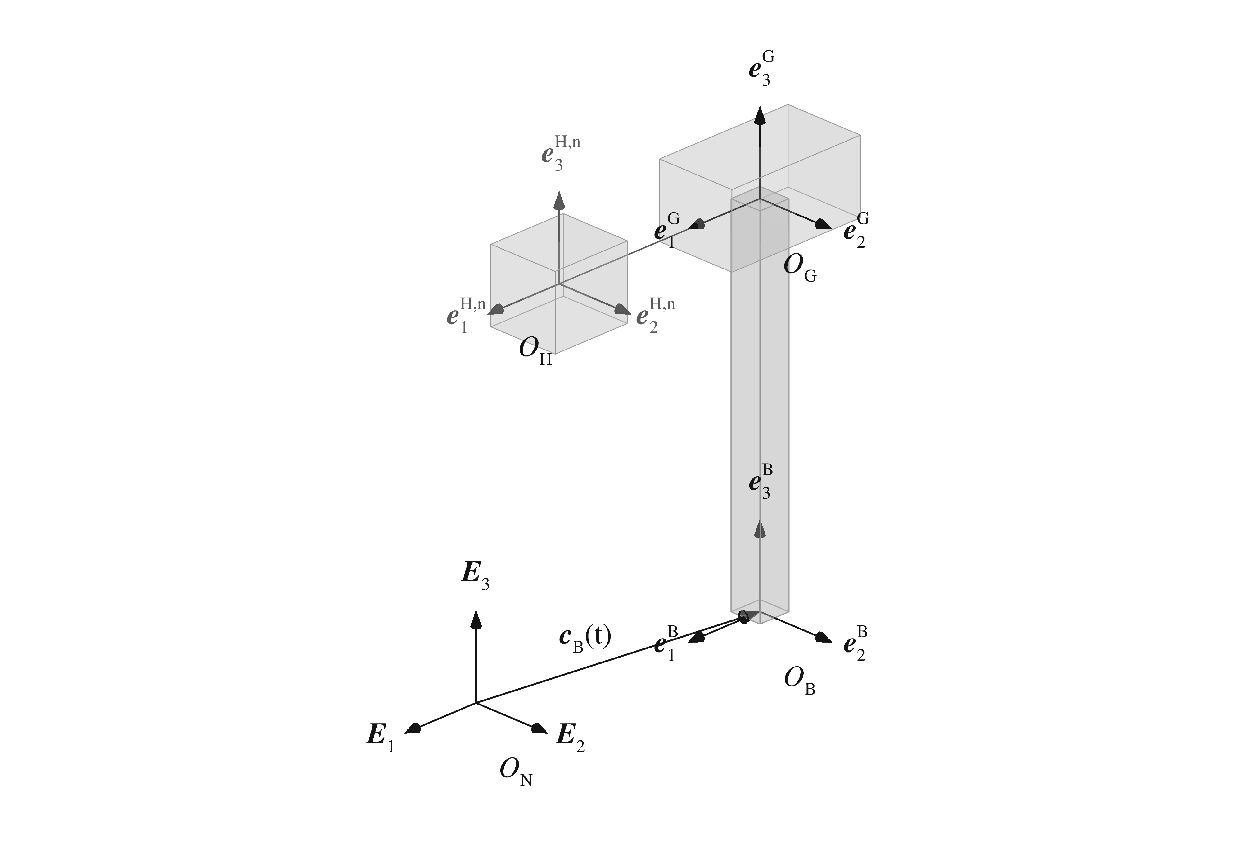
\includegraphics[width=.96\linewidth,height=.40\textheight,keepaspectratio]{figures/tecplot/concept_sistemas-lateral.pdf}
\caption[Sistemas de referencia de la base y la góndola]{Sistemas de referencia de la base, la góndola y el cubo en una vista espacial. $\vct c_B(t)$ sitúa la base respecto de $O_N$ y los triedros muestran sus tres direcciones. El superíndice $H,n$ identifica la base nominal del cubo. Los volúmenes y separaciones son esquemáticos; no representan una malla de sólidos.}\label{fig:sistemas-lateral}
\end{figure}

\begin{figure}[htbp]
\centering
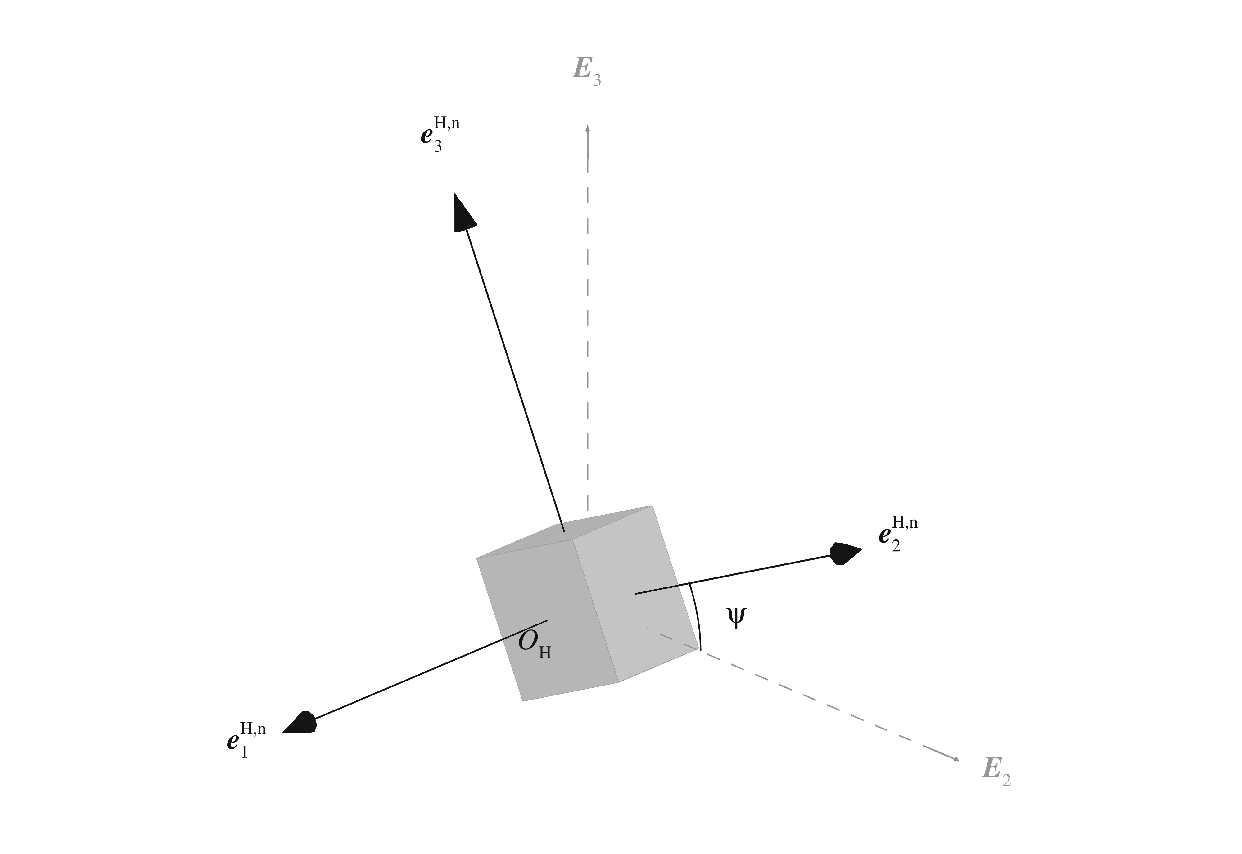
\includegraphics[width=.96\linewidth,height=.40\textheight,keepaspectratio]{figures/tecplot/concept_cubo-nominal.pdf}
\caption[Rotación nominal del cubo]{Orientación nominal del cubo en tres dimensiones. El azimut $\psi$ gira las direcciones 2 y 3 alrededor del eje 1, que permanece común. Las direcciones inerciales son discontinuas y las nominales continuas. El superíndice $H,n$ equivale a la notación $\overline{\vct e}_i^H$ del texto.}\label{fig:cubo-nominal}
\end{figure}

\subsection{Sistemas de referencia de las tres palas}
Cada pala $b\in\{1,2,3\}$ tiene un sistema de referencia de montaje $\mathcal F_{P_b}$ en su raíz. Para espaciamiento uniforme, $\beta_b=2\pi(b-1)/3$. La orientación nominal es
\begin{equation}
 {}^N\overline Q_{P_b}(t)={}^N\overline Q_H(t){}^HQ_{P_b},
 \qquad {}^HQ_{P_b}=R_1(\beta_b)Q_{\rm mont,b}.
\end{equation}
La matriz $Q_{\rm mont,b}$ establece la orientación de la sección de raíz. Para tres palas rectas sin cono ni paso inicial, se adopta la misma matriz de montaje antes de aplicar la separación angular de cada pala:
\begin{equation}
 Q_{\rm mont,b}=[\vct e_3,-\vct e_2,\vct e_1],
 \qquad\text{componentes expresadas en }H.
\end{equation}
Así, el eje 1 de cada pala es radial, el eje 2 es tangencial en el sentido de giro positivo y el eje 3 es paralelo al eje del rotor. La pala 1 coincide con el eje 3 del cubo cuando $\psi=0$; para una góndola horizontal, apunta verticalmente hacia arriba. Esta elección coincide con las vistas de las figuras~\ref{fig:turbina} y \ref{fig:cubo-brazos}.

Las direcciones nominales, expresadas en el cubo, quedan definidas por
\begin{align}
 \vct d_{1b}^H&=-\sin\beta_b\,\vct e_2+\cos\beta_b\,\vct e_3,\\
 \vct d_{2b}^H&=-\cos\beta_b\,\vct e_2-\sin\beta_b\,\vct e_3,
 &\vct d_{3b}^H&=\vct e_1.
\end{align}
En particular, las matrices de las tres palas son
\begin{align}
 {}^HQ_{P_1}&=\begin{bmatrix}0&0&1\\0&-1&0\\1&0&0\end{bmatrix},\\
 {}^HQ_{P_2}&=\begin{bmatrix}
 0&0&1\\-\sqrt3/2&1/2&0\\-1/2&-\sqrt3/2&0
 \end{bmatrix},\qquad
 {}^HQ_{P_3}=\begin{bmatrix}
 0&0&1\\\sqrt3/2&1/2&0\\-1/2&\sqrt3/2&0
 \end{bmatrix}.
 \label{eq:matrices-tres-palas}
\end{align}
Si $r_H$ es la distancia del centro del cubo a cada raíz, sus posiciones relativas son
\begin{equation}
 \vct r_{10}^H=r_H\begin{bmatrix}0\\0\\1\end{bmatrix},\quad
 \vct r_{20}^H=r_H\begin{bmatrix}0\\-\sqrt3/2\\-1/2\end{bmatrix},\quad
 \vct r_{30}^H=r_H\begin{bmatrix}0\\\sqrt3/2\\-1/2\end{bmatrix}.
 \label{eq:raices-tres-palas}
\end{equation}
Estos vectores describen posiciones, mientras que las columnas de \eqref{eq:matrices-tres-palas} describen direcciones unitarias. Multiplicar los primeros por la orientación del cubo sitúa las raíces en el espacio; multiplicar las matrices por esa orientación determina los ejes de cada pala.

La figura~\ref{fig:marcos} identifica simultáneamente las nueve direcciones locales de las tres raíces. Las tres direcciones $\vct d_{3b}^H$ coinciden con el eje del rotor; las seis direcciones restantes se leen en el plano. Los puntos de raíz son distintos aunque pertenezcan al mismo cuerpo rígido de unión.
\begin{figure}[htbp]
\centering
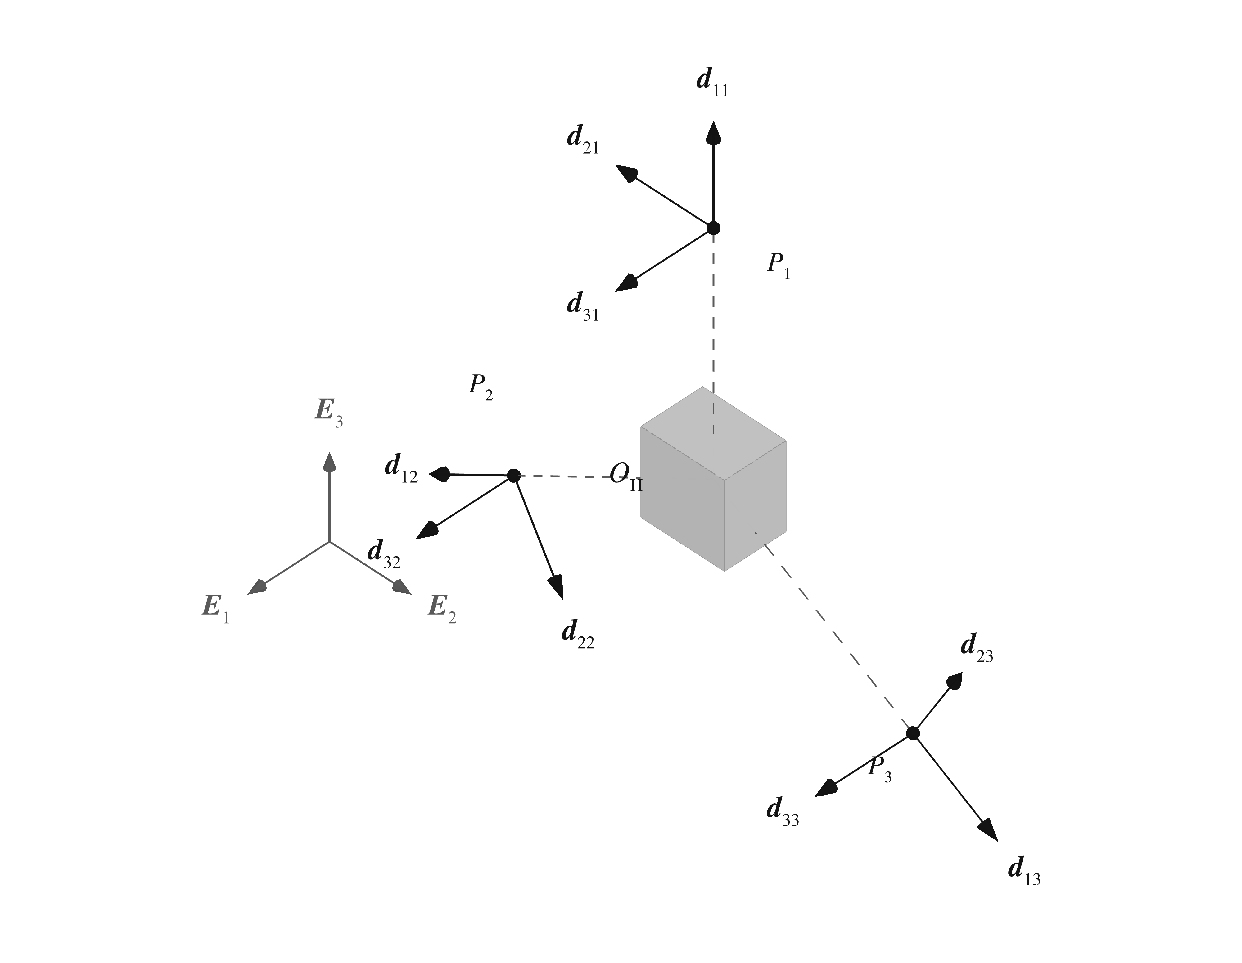
\includegraphics[width=.96\linewidth,height=.40\textheight,keepaspectratio]{figures/tecplot/concept_marcos.pdf}
\caption[Sistemas de referencia de las raíces]{Triedros de las tres raíces para azimut nominal nulo. El eje $\vct d_{1b}$ es longitudinal, $\vct d_{2b}$ tangencial y $\vct d_{3b}=\vct E_1$. Se muestran las tres direcciones, los puntos $P_b$ y el origen del cubo. Las separaciones angulares son $120^\circ$ y la perspectiva conserva la convención dextrógira.}\label{fig:marcos}
\end{figure}

Un paso fijo $\alpha_{p,b}$ se incorpora por una rotación alrededor del eje longitudinal de la pala:
\begin{equation}
 {}^HQ_{P_b}^{\,\mathrm{paso}}
 ={}^HQ_{P_b}R_1(\alpha_{p,b}).
 \label{eq:paso-fijo}
\end{equation}
El ángulo de paso orienta la sección en la raíz; la torsión geométrica describe la variación de esa orientación a lo largo de la pala; y la torsión elástica es el cambio producido por la deformación. Son tres magnitudes distintas. En el movimiento nominal adoptado, el paso es constante y no aporta una velocidad angular relativa. La torsión elástica, cuando varía con el tiempo, sí contribuye a la velocidad angular de las secciones.

La figura~\ref{fig:palas-paso} muestra el ángulo de paso en el plano de la sección, separado del azimut del rotor.

\begin{figure}[htbp]
\centering
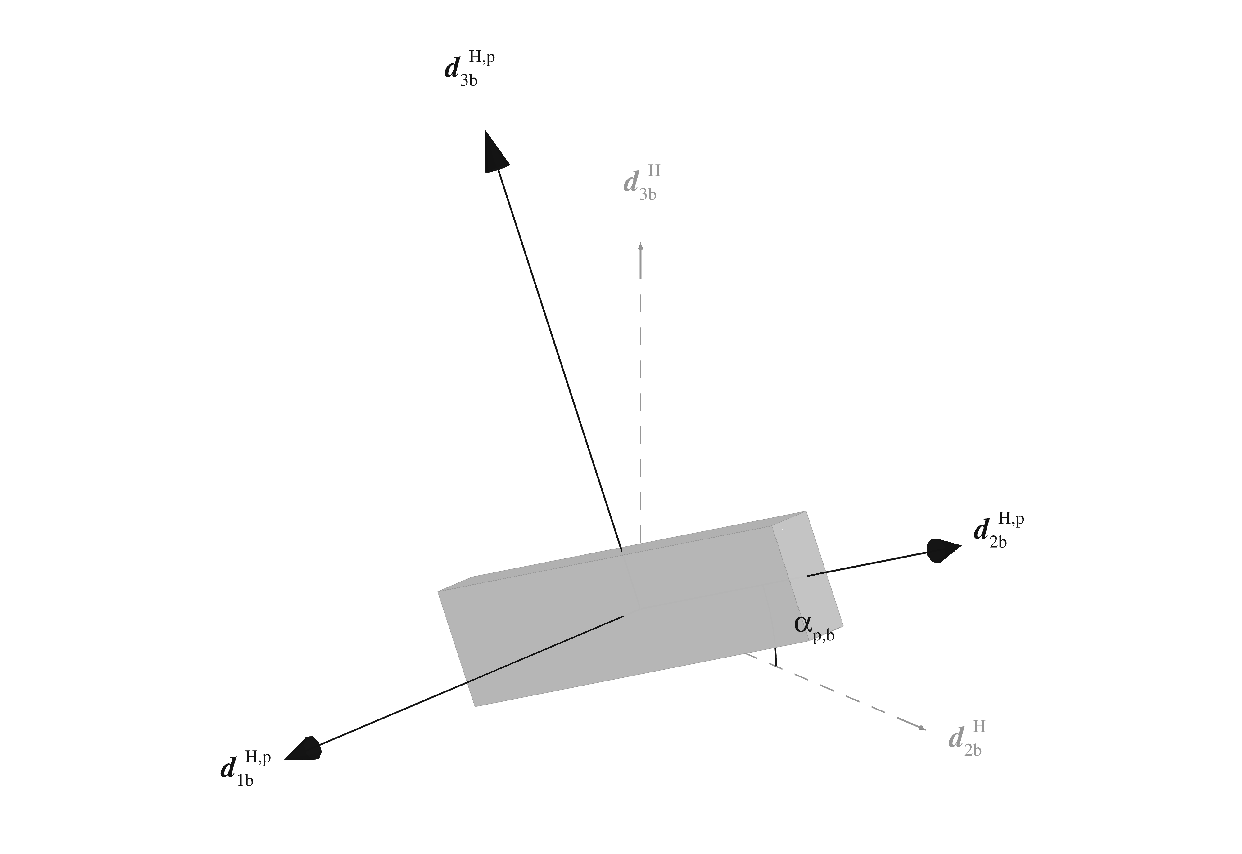
\includegraphics[width=.96\linewidth,height=.40\textheight,keepaspectratio]{figures/tecplot/concept_palas-paso.pdf}
\caption[Ángulo de paso de una sección de pala]{Rotación de paso de una sección en tres dimensiones. Las direcciones discontinuas $\vct d_{ib}^{H}$ corresponden al montaje sin paso y las continuas $\vct d_{ib}^{H,p}$ a la sección rotada. El eje longitudinal permanece común y la raíz no se traslada. El espesor de la sección facilita la lectura de su orientación.}\label{fig:palas-paso}
\end{figure}

Las relaciones entre los sistemas de referencia se reúnen en la figura~\ref{fig:arbol}; esta organización permite construir a continuación la posición absoluta de cada componente.

\begin{figure}[htbp]
\centering
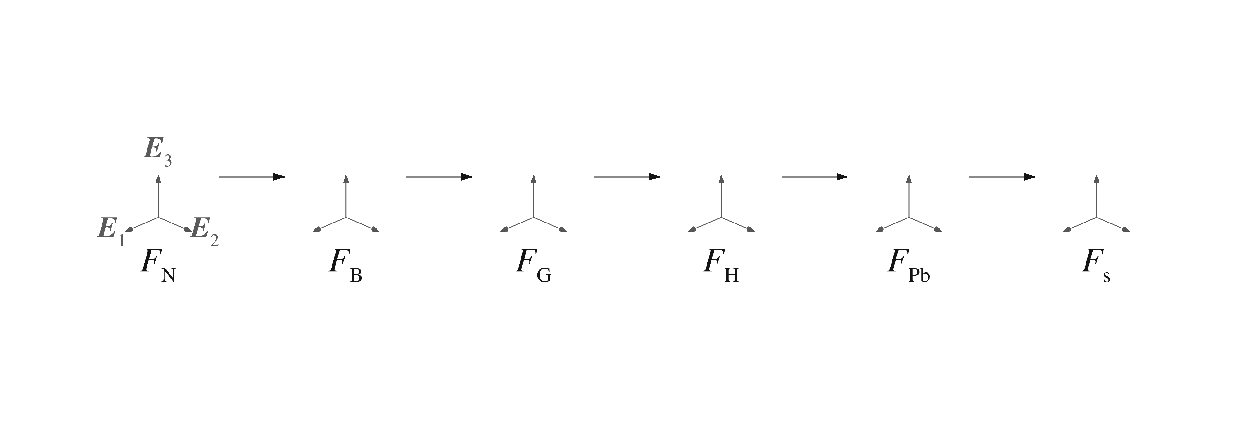
\includegraphics[width=.96\linewidth,height=.40\textheight,keepaspectratio]{figures/tecplot/concept_arbol.pdf}
\caption[Relaciones entre los sistemas de referencia]{Jerarquía de los sistemas de referencia: newtoniano $N$, base $B$, góndola $G$, cubo $H$, raíz $P_b$ y sección $s$. Cada símbolo $\mathcal F$ identifica un triedro espacial. Las flechas indican relaciones cinemáticas y cambios de componentes; las ubicaciones son esquemáticas y no imponen conexiones rígidas.}\label{fig:arbol}
\end{figure}

\subsection{Construcción explícita de las posiciones de los componentes}
Los sistemas de referencia anteriores permiten escribir posiciones sin ambigüedad. Para una partícula de la torre, con $\vct R_T(S)=S\vct E_3$ en la referencia recta, se usa
\begin{equation}
 \vct x_T=\vct c_B(t)+\vct R_T(S)+\vct u_T(S,t)
 +\xi_2\vct d_{2T}(S,t)+\xi_3\vct d_{3T}(S,t).
\end{equation}
Aquí $\vct u_T$ es el desplazamiento de la línea de torre relativo a la base. La traslación sísmica $\vct u_B$ aparece una sola vez, en $\vct c_B$. Para una góndola rígida,
\begin{equation}
 \vct x_G=\vct c_G(t)+{}^NQ_G(t)\vct\rho_G,
\end{equation}
donde $\vct\rho_G$ identifica una partícula respecto del punto de referencia elegido en el cuerpo. Si la góndola está soldada a la sección superior de torre, $\vct c_G$ y ${}^NQ_G$ se deducen de esa sección y de la separación geométrica de montaje. Si existe una unión flexible, la diferencia relativa constituye una incógnita y la unión aporta una relación constitutiva entre acciones y desplazamientos relativos, no una identidad cinemática.

Para el cubo--nariz rígido se escribe análogamente
\begin{equation}
 \vct x_H=\vct c_H(t)+{}^NQ_H(t)\vct\rho_H,
 \qquad {}^NQ_H={}^N\overline Q_H\exp([\vct\theta_H]_\times).
\end{equation}
El vector $\vct\rho_H$ permanece fijo en el cuerpo; $\vct\theta_H$ es una perturbación respecto del giro nominal. Se distingue de $\psi$, que puede recorrer muchas revoluciones. La nariz comparte esta expresión solamente bajo la idealización rígida conjunta declarada.

Una pala se describe en su propio sistema de referencia de raíz: $\vct r_b^P(S,t)$ es la posición de su línea respecto a la raíz y $\vct d_{\alpha b}^P$ son sus directores. La posición absoluta de una partícula resulta
\begin{equation}
 \vct x_b=\vct c_{P_b}(t)+{}^NQ_{P_b}(t)
 \left[\vct r_b^P(S,t)+\xi_2\vct d_{2b}^P+\xi_3\vct d_{3b}^P\right].
\end{equation}
En una raíz soldada, $\vct c_{P_b}=\vct c_H+{}^NQ_H\vct r_{b0}^H$ y ${}^NQ_{P_b}={}^NQ_H{}^HQ_{P_b}$, con $\vct r_{b0}^H$ fijo. Entonces se elige $\vct r_b^P(0,t)=0$ y la orientación relativa de raíz coincide con el montaje. La deformación de las secciones interiores sigue siendo libre. Estas expresiones describen campos continuos; imponer su versión nodal corresponde al capítulo de elementos finitos.

La figura~\ref{fig:cadena-posiciones} representa la suma de posiciones de la ecuación anterior, desde el origen newtoniano hasta la partícula de pala.

\begin{figure}[htbp]
\centering
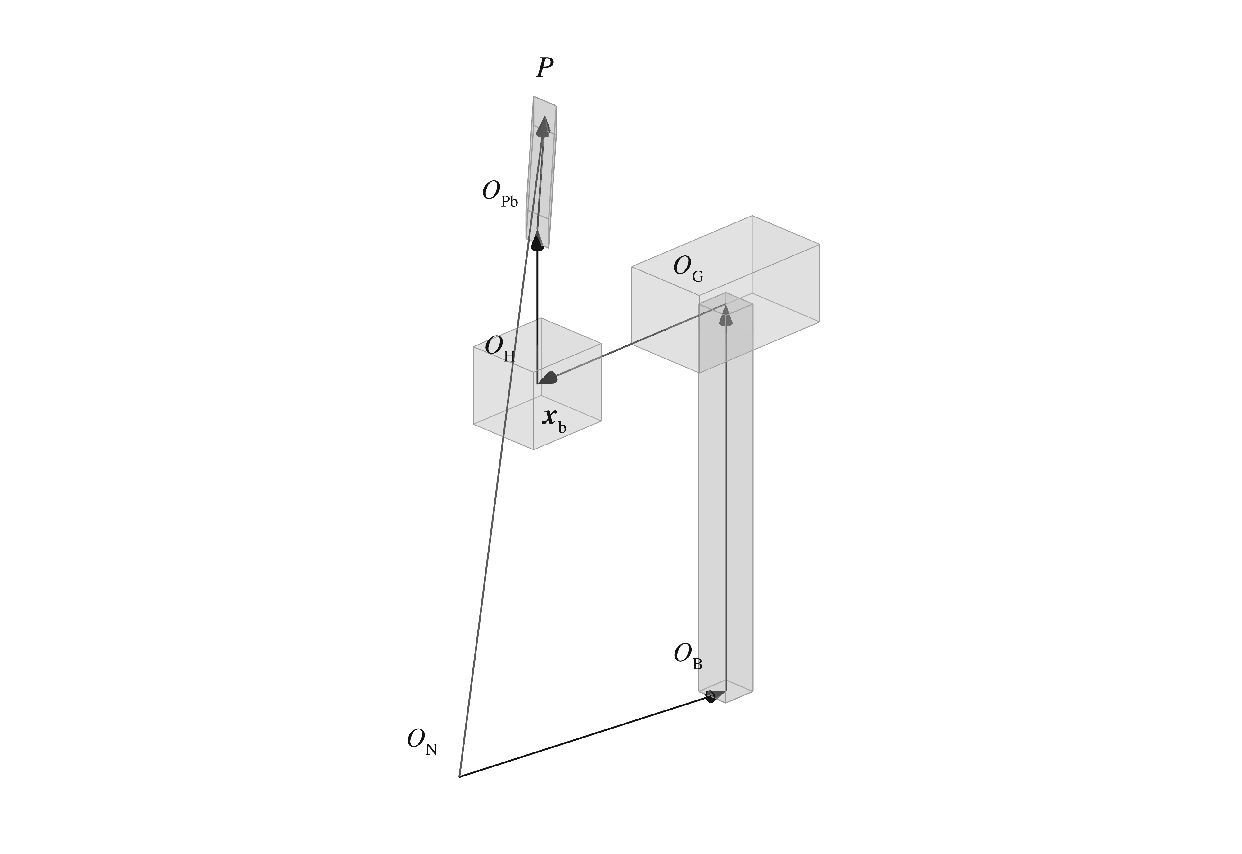
\includegraphics[width=.96\linewidth,height=.40\textheight,keepaspectratio]{figures/tecplot/concept_cadena-posiciones.pdf}
\caption[Composición de posiciones]{Composición de posiciones desde el origen newtoniano hasta una partícula de pala. Los puntos intermedios corresponden a la base, la góndola, el cubo y la raíz. La flecha directa representa la posición absoluta $\vct x_b$. El esquema espacial no está a escala.}\label{fig:cadena-posiciones}
\end{figure}

\section{Movimiento nominal y configuración deformada}
\subsection{Configuración de referencia, movimiento nominal y configuración actual}
Para una partícula del rotor puede definirse un movimiento nominal rígido
\begin{equation}
 \overline{\vct\chi}(\vct X,t)=\overline{\vct c}_H(t)
 +{}^N\overline Q_H(t)\vct a(\vct X),
\end{equation}
donde $\vct a$ es su posición material relativa al cubo en coordenadas nominales. Si se añaden deformaciones, el movimiento actual será
\begin{equation}
 \vct\chi(\vct X,t)=\overline{\vct c}_H(t)+{}^N\overline Q_H(t)
 [\vct a(\vct X)+\vct u_c(\vct X,t)].
 \label{eq:nominalactual}
\end{equation}
El subíndice $c$ indica componentes en el sistema de referencia nominal corrotante, no que el material permanezca rígido. La deformación operativa, por ejemplo debida a las cargas medias, puede incluirse en $\vct u_c=\vct u_{c0}+\widetilde{\vct u}_c$. La tilde denota una perturbación alrededor de esa deformación operativa.

La configuración de referencia identifica las partículas mediante sus coordenadas materiales. El movimiento nominal describe la traslación y la rotación prescritas de esa geometría. El estado de operación incorpora las deformaciones asociadas a las cargas y al giro, y la configuración actual contiene además la perturbación vibratoria. Estas definiciones permiten describir una misma partícula desde la geometría inicial hasta su posición durante la operación.

En la figura~\ref{fig:tresniveles}, $\overline{\mathcal B}_t$ denota la configuración ocupada bajo el movimiento nominal y $\overline{\vct x}=\overline{\vct\chi}(\vct X,t)$. La diferencia de posiciones se expresa en ejes inerciales: $\vct x-\overline{\vct x}={}^N\overline Q_H\vct u_c$. La traslación nominal del cubo aparece en ambas posiciones y se cancela en esa diferencia.
\begin{figure}[htbp]
\centering
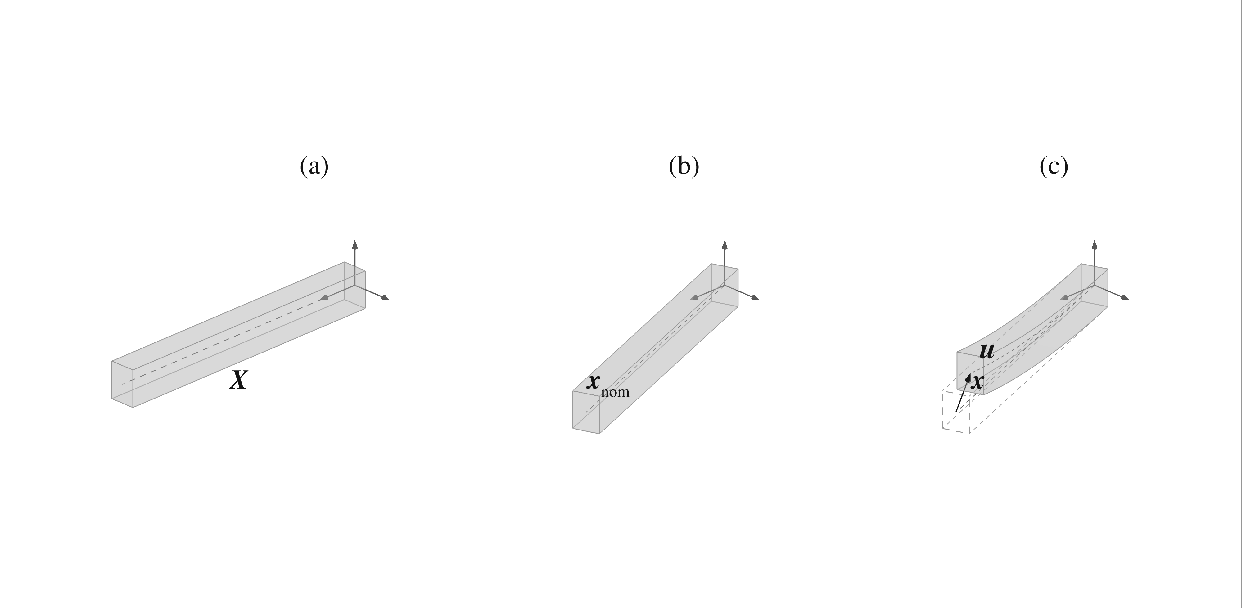
\includegraphics[width=.96\linewidth,height=.40\textheight,keepaspectratio]{figures/tecplot/concept_tresniveles.pdf}
\caption[Referencia material, movimiento nominal y perturbación]{Una misma porción de viga en (a) referencia material, (b) movimiento nominal y (c) configuración actual. El contorno discontinuo de (c) reproduce la configuración nominal; la diferencia se identifica mediante $\vct u$. Los pequeños triedros conservan la orientación inercial en los tres paneles.}\label{fig:tresniveles}
\end{figure}

\subsection{Giro prescrito y grados de libertad estructurales}
Al suprimir las deformaciones del rotor, su movimiento nominal se describe por un solo parámetro angular. Como $\psi(t)$ está dado, ese parámetro no se cuenta entre las incógnitas dinámicas. La turbina completa no se convierte en un sólido de un grado de libertad: permanecen la torre estacionaria, las conexiones y, cuando se restituyen, las múltiples perturbaciones estructurales.

Una perturbación torsional del eje representa una desviación respecto del giro prescrito. Si se incluye y existe rigidez torsional, no es un mecanismo libre. Si se elimina por una restricción de velocidad ideal, no debe aparecer como incógnita adicional. La elección depende de la representación del tren de potencia y debe declararse antes del análisis modal.

\section{Cinemática continua de una viga espacial}
\subsection{Línea de referencia y directores}
Se parametriza la viga por una coordenada material $S\in[0,L]$ y dos coordenadas transversales $\xi_2,\xi_3$. En referencia,
\begin{equation}
 \vct X(S,\xi_2,\xi_3)=\vct R(S)+\xi_2\vct D_2(S)+\xi_3\vct D_3(S).
\end{equation}
La línea $\vct R(S)$ une los puntos de referencia de las secciones. Los directores $\vct D_i$ son unitarios y ortogonales, con $\vct D_1=\vct D_2\times\vct D_3$. En la configuración actual, bajo la hipótesis de sección rígida,
\begin{equation}
 \vct x(S,\xi_2,\xi_3,t)=\vct r(S,t)+\xi_2\vct d_2(S,t)+\xi_3\vct d_3(S,t).
 \label{eq:beamkin}
\end{equation}
La misma partícula conserva $S,\xi_2,\xi_3$. La hipótesis excluye deformación dentro del plano de la sección y alabeo explícito, pero admite su traslación y orientación independientes. El efecto del alabeo de torsión puede incorporarse en una rigidez seccional efectiva sin resolverlo como campo cinemático adicional.

El punto $\vct r(S,t)$ es el origen elegido para una sección, no necesariamente su centro de masa ni su centro geométrico. Los directores $\vct d_2$ y $\vct d_3$ indican las direcciones de las coordenadas transversales. El director $\vct d_1=\vct d_2\times\vct d_3$ completa la base ortonormal y es normal a la sección. La posición de una partícula se reconstruye sumando la posición del origen seccional y los dos vectores transversales. De esta manera, las tres coordenadas materiales identifican una partícula del volumen, mientras que los campos $\vct r$ y $Q$ describen el movimiento de toda la viga.

La figura~\ref{fig:particula-seccion} separa la posición del origen seccional de la posición de la partícula dentro de esa sección.

\begin{figure}[htbp]
\centering
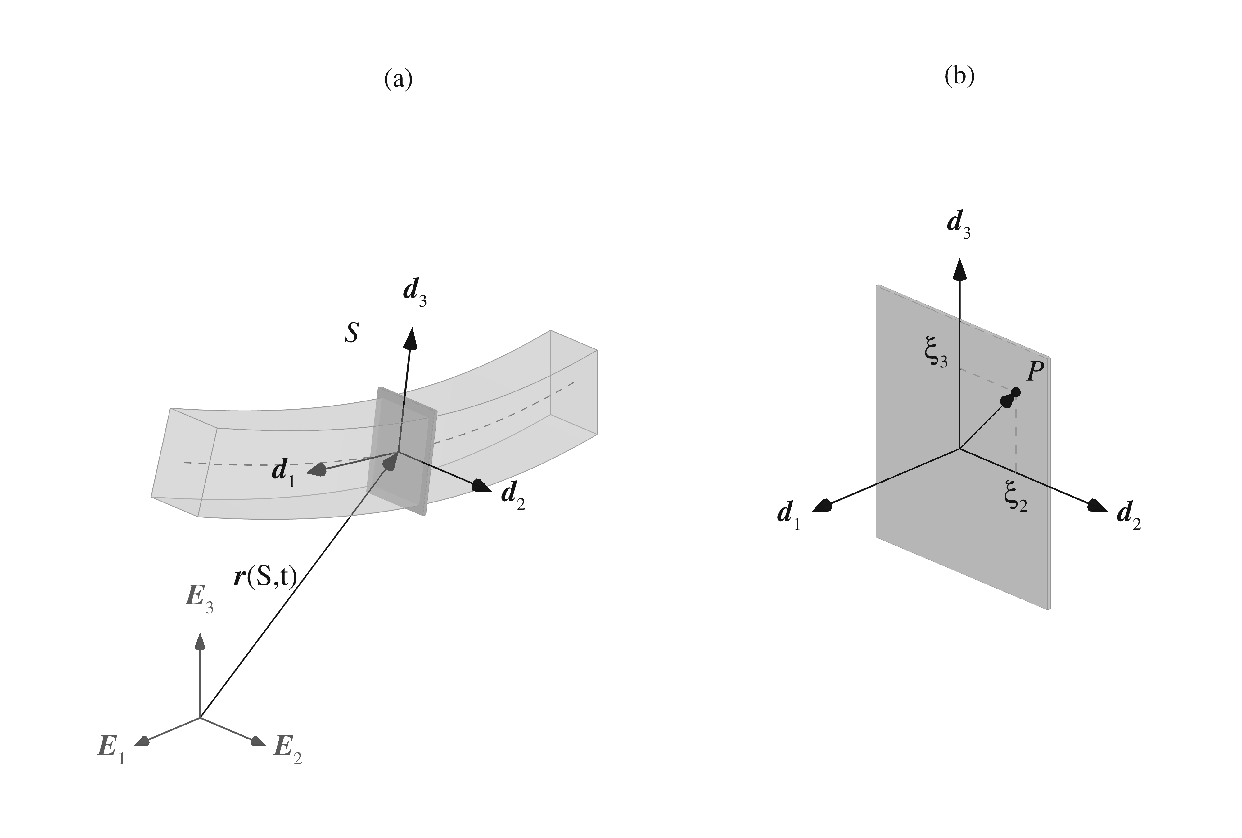
\includegraphics[width=.96\linewidth,height=.40\textheight,keepaspectratio]{figures/tecplot/concept_particula-seccion.pdf}
\caption[Posición de una partícula de viga]{Posición de una partícula de viga. (a) Línea de referencia $\vct r(S,t)$, sección rígida y triedro de directores. (b) Ampliación de la sección: $\vct x_P=\vct r+\xi_2\vct d_2+\xi_3\vct d_3$. Se muestran los tres directores; $\vct d_1$ es normal a la sección. El volumen transparente representa la envolvente de la viga.}\label{fig:particula-seccion}
\end{figure}

Sean $Q_0=[\vct D_1,\vct D_2,\vct D_3]$ y $Q=[\vct d_1,\vct d_2,\vct d_3]$ en componentes newtonianas. Ambas matrices pertenecen a $\SO$. La rotación física que lleva los directores iniciales a los actuales es $QQ_0^\tr$.

\subsection{Extensión y cortante}
Con prima indicando derivada respecto de $S$, se define
\begin{equation}
 \vct\gamma=Q^\tr\vct r'-Q_0^\tr\vct R'.
 \label{eq:gamma}
\end{equation}
Esta terna expresa el cambio del vector tangente medido por la propia sección. Si $S$ es longitud de arco de referencia y $\vct R'=\vct D_1$, el segundo término es $(1,0,0)^\tr$. La componente $\gamma_1$ representa extensión de la línea, mientras $\gamma_2$ y $\gamma_3$ describen cortante. El director $\vct d_1$ no se impone paralelo a $\vct r'$. Imponerlo anularía el cortante y cambiaría la teoría de viga.

La figura~\ref{fig:shear} muestra la diferencia entre la normal a la sección y la tangente a la línea deformada, que da lugar a la deformación por cortante.

\begin{figure}[htbp]
\centering
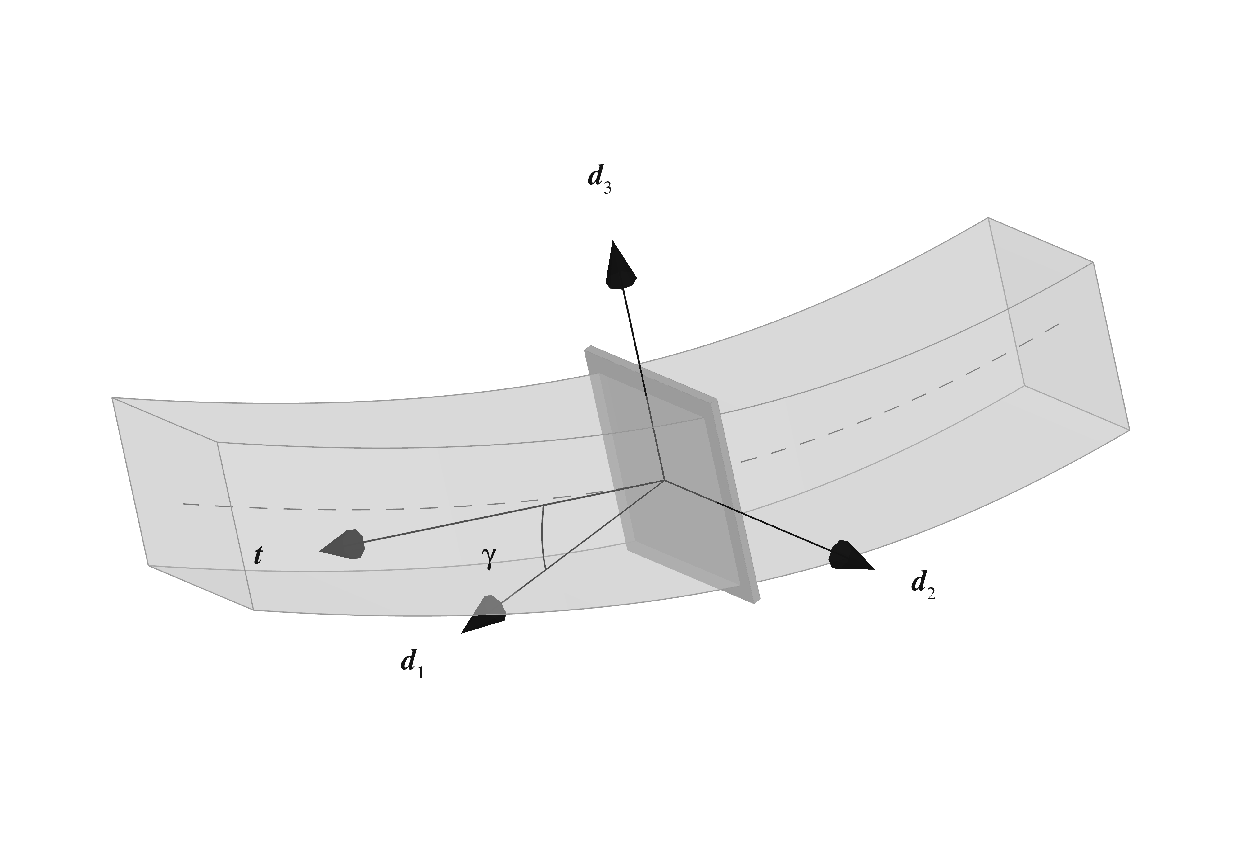
\includegraphics[width=.96\linewidth,height=.40\textheight,keepaspectratio]{figures/tecplot/concept_shear.pdf}
\caption[Normal a la sección y tangente a la línea]{Normal $\vct d_1$ a la sección y tangente $\vct t$ a la línea de referencia de una viga con cortante. El arco $\gamma$ mide el ángulo entre ambas direcciones en el esquema espacial. La rigidez de la sección no obliga a que su normal coincida con la tangente.}\label{fig:shear}
\end{figure}

\subsection{Curvatura y torsión}
Como $Q^\tr Q=\Id$, la matriz $Q^\tr Q'$ es antisimétrica. Se define
\begin{equation}
 \vct\kappa=\ax(Q^\tr Q')-\ax(Q_0^\tr Q_0').
 \label{eq:kappa}
\end{equation}
Su primera componente mide torsión y las otras dos flexión. Se resta la curvatura material inicial para que una geometría precurvada sin deformación no produzca curvatura elástica. Las componentes se interpretan con respecto a las mismas etiquetas materiales de los directores.

Estas medidas son objetivas ante una traslación y rotación rígida superpuestas: si $\vct r^*=\vct c+P\vct r$, $Q^*=PQ$ y $P$ no depende de $S$, entonces $(Q^*)^\tr(\vct r^*)'=Q^\tr\vct r'$ y $(Q^*)^\tr(Q^*)'=Q^\tr Q'$. Un movimiento rígido no cambia $\vct\gamma$ ni $\vct\kappa$. Esta invariancia permite conservar el giro nominal sin atribuirle deformaciones espurias.

\subsection{Relación con el gradiente tridimensional}
La reducción de viga puede conectarse con $\ten F$ sin introducir nodos. Definiendo
\begin{align}
 \vct G_1&=\vct R'+\xi_2\vct D_2'+\xi_3\vct D_3',&
 \vct G_2&=\vct D_2,&\vct G_3&=\vct D_3,\\
 \vct g_1&=\vct r'+\xi_2\vct d_2'+\xi_3\vct d_3',&
 \vct g_2&=\vct d_2,&\vct g_3&=\vct d_3,
\end{align}
y la base recíproca $\vct G^i\cdot\vct G_j=\delta^i_j$, se obtiene $\ten F=\vct g_i\otimes\vct G^i$. La necesidad de base recíproca explica por qué no se puede tratar sin más una parametrización curva como cartesiana. El modelo unidimensional conserva ciertas deformaciones del continuo y elimina otras por hipótesis.

\section{Rotaciones finitas y perturbaciones pequeñas}
\subsection{Representación exponencial}
La orientación perturbada de un triedro nominal $\overline Q$ se escribe
\begin{equation}
 Q=\overline Q E(\vct\theta),\qquad E(\vct\theta)=\exp(\sk\theta).
 \label{eq:exprot}
\end{equation}
Las componentes de $\vct\theta$ están en la base nominal que precede a $E$. Para $\vartheta=\|\vct\theta\|$, la fórmula de Rodrigues es
\begin{equation}
 E=\Id+\frac{\sin\vartheta}{\vartheta}\sk\theta
 +\frac{1-\cos\vartheta}{\vartheta^2}\sk\theta^2,
\end{equation}
con límites continuos en cero. El vector de rotación es una parametrización local; no es una terna de ángulos de Euler. Dos rotaciones finitas se componen multiplicando sus matrices, no sumando sus vectores. A primer orden, $E\simeq\Id+\sk\theta$, y solo en ese régimen las sumas de pequeños incrementos son compatibles con una aproximación lineal.

En la figura~\ref{fig:giro-perturbacion} se presenta un caso particular que permite separar visualmente las dos rotaciones: tanto el giro nominal como la perturbación se toman alrededor del eje 1. En ese caso especial sus ángulos pueden sumarse. Para una perturbación general, sus tres componentes se incorporan mediante el producto matricial~\eqref{eq:exprot}; el dibujo no justifica sumar ángulos alrededor de ejes diferentes.

\begin{figure}[htbp]
\centering
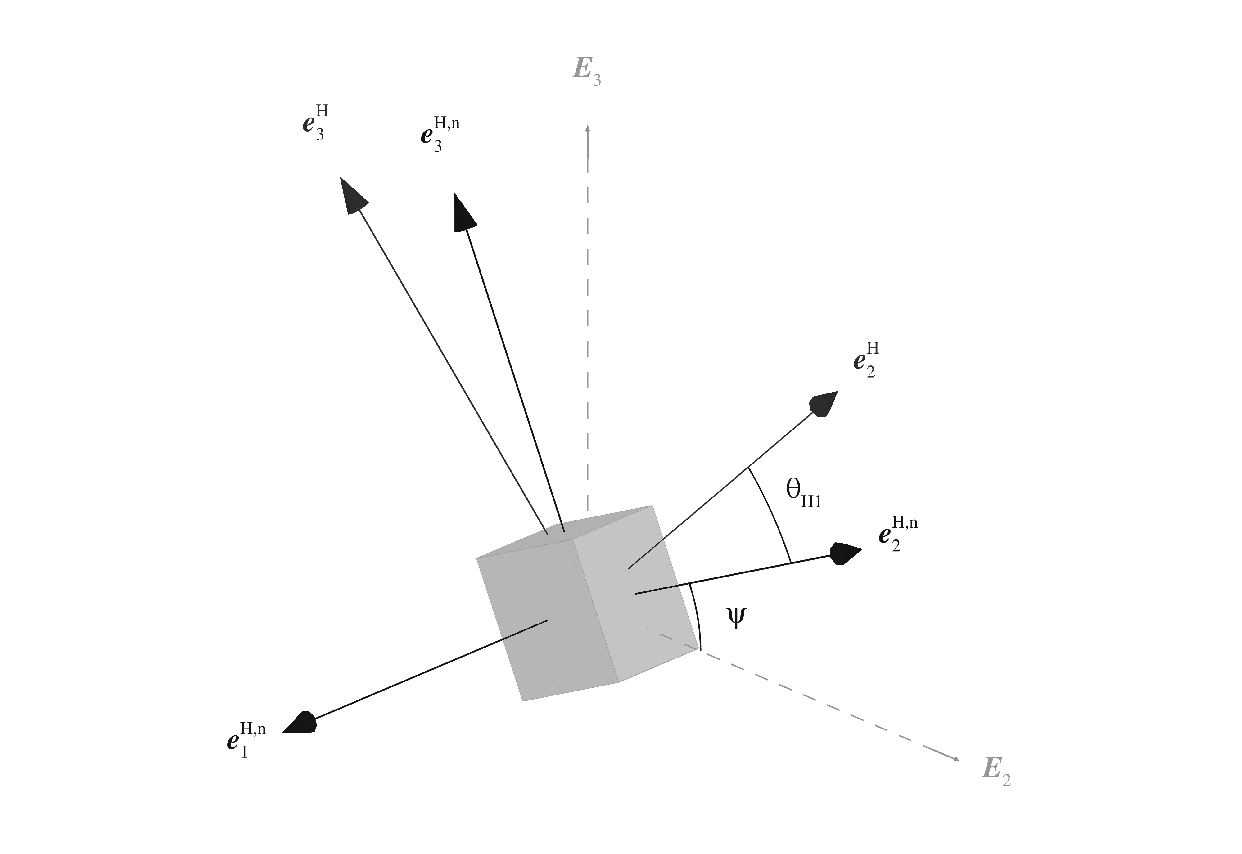
\includegraphics[width=.96\linewidth,height=.40\textheight,keepaspectratio]{figures/tecplot/concept_giro-perturbacion.pdf}
\caption[Rotación nominal y perturbación angular]{Separación de la orientación inercial, la rotación nominal $\psi$ y una perturbación rotacional del cubo. El superíndice $H,n$ indica la base nominal y $H$ la perturbada. El incremento $\theta_{H1}$ se amplía para distinguir los triedros; la formulación emplea pequeñas perturbaciones.}\label{fig:giro-perturbacion}
\end{figure}

\subsection{Velocidad angular y derivada del vector de rotación}
En general $\dot{\vct\theta}$ no es la velocidad angular exacta. La identidad
\begin{equation}
 \dot E E^\tr=\sk{J_\ell(\vct\theta)\dot{\vct\theta}},\quad
 J_\ell(\vct\theta)=\Id+
 \frac{1-\cos\vartheta}{\vartheta^2}\sk\theta+
 \frac{\vartheta-\sin\vartheta}{\vartheta^3}\sk\theta^2
\end{equation}
define el Jacobiano izquierdo de la parametrización exponencial. En particular,
\begin{equation}
 J_\ell\dot{\vct\theta}=\dot{\vct\theta}
 +\tfrac12\vct\theta\times\dot{\vct\theta}+O(\epsilon^3)
\end{equation}
si $\vct\theta$ y su derivada son de orden $\epsilon$. El término cuadrático puede contribuir a las ecuaciones lineales al multiplicarse por una velocidad nominal no nula en la energía cinética. Por ello no siempre es correcto linealizar todas las velocidades antes de formar la energía que se va a expandir.

\subsection{Límite de pequeñas deformaciones de una viga recta}
Para una viga inicialmente recta en el eje local 1, con $Q_0=\Id$, se toma $\vct r=(S,0,0)^\tr+\vct u$ y $Q\simeq\Id+\sk\theta$. Al retener primer orden,
\begin{equation}
 \vct\gamma=\vct u'-\vct\theta\times\vct e_1,
 \qquad \vct\kappa=\vct\theta'.
\end{equation}
Como $\vct\theta\times\vct e_1=(0,\theta_3,-\theta_2)^\tr$, se obtiene
\begin{equation}
 \vct e_s=
 [u_1',\ u_2'-\theta_3,\ u_3'+\theta_2,\ \theta_1',\ \theta_2',\ \theta_3']^\tr.
 \label{eq:strainlinear}
\end{equation}
Esta expresión fija los signos que se emplearán al construir la matriz deformación--desplazamiento. Aún no hay nodos: $\vct u(S,t)$ y $\vct\theta(S,t)$ son campos continuos.

\section{Velocidades y aceleraciones en el sistema giratorio}
\subsection{Posición y velocidad de una partícula}
Sea $Q_c(t)={}^N\overline Q_H(t)$ y $\vct y(t)$ la posición relativa de una partícula en ese sistema de referencia. Definimos $\vct\Omega_c=\Omega\vct e_1$ y $W=\sk{\Omega_c}$, de manera que $\dot Q_c=Q_cW$. La posición y velocidad absolutas son
\begin{align}
 \vct x&=\vct c(t)+Q_c(t)\vct y(t),\\
 \dot{\vct x}&=\dot{\vct c}+Q_c(\dot{\vct y}+W\vct y).
 \label{eq:velocitytransport}
\end{align}
El término $Q_c\dot{\vct y}$ es velocidad relativa transportada a la base newtoniana. El término $Q_cW\vct y$ existe aunque la partícula esté fija en el sistema de referencia giratorio. La suma se realiza después de expresar ambos en una base común.

La suma de la ecuación~\eqref{eq:velocitytransport} se representa en la figura~\ref{fig:suma-velocidades}. No se suman velocidades medidas por observadores diferentes sin transformar sus componentes. Cada lado del polígono es ya una velocidad expresada en el sistema newtoniano.

\begin{figure}[htbp]
\centering
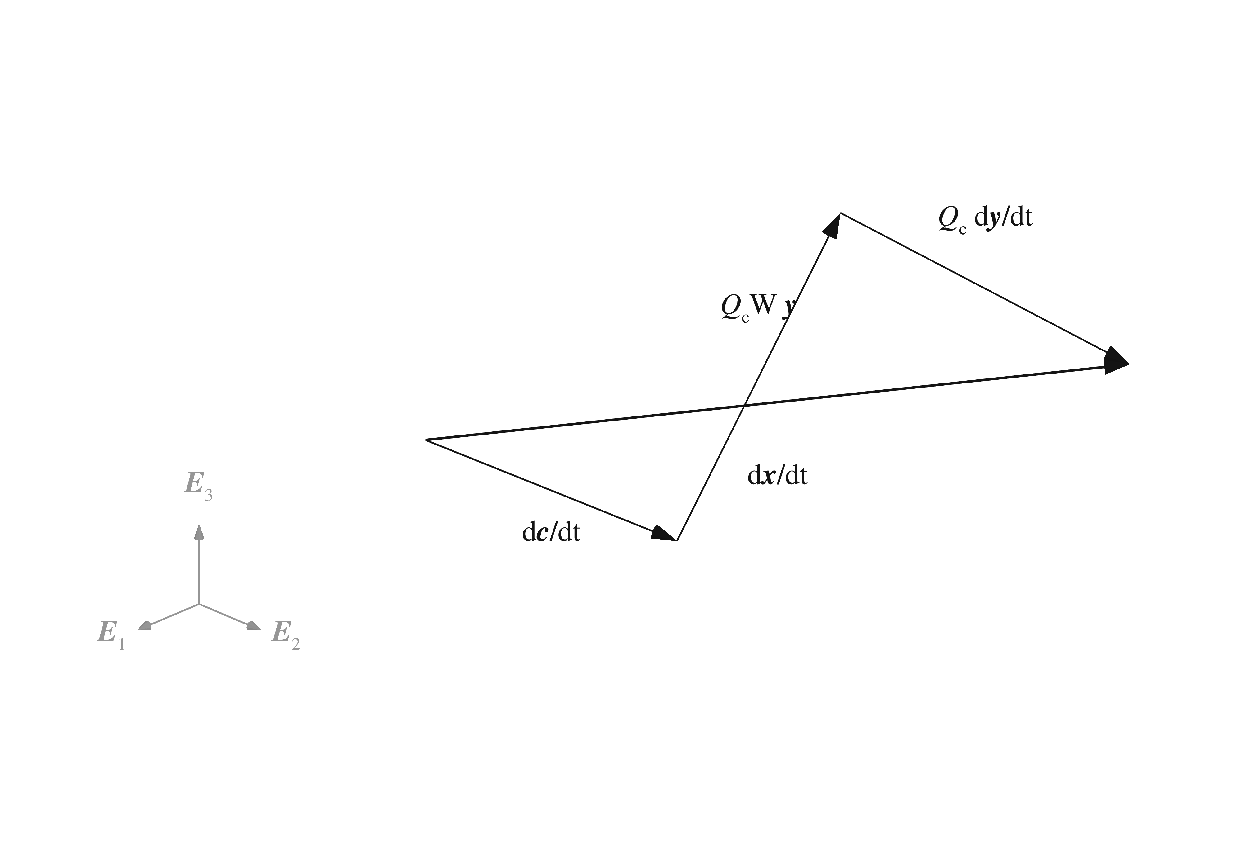
\includegraphics[width=.96\linewidth,height=.40\textheight,keepaspectratio]{figures/tecplot/concept_suma-velocidades.pdf}
\caption[Composición de velocidades]{Suma vectorial de los tres términos del teorema de transporte. Las flechas sucesivas representan la velocidad de traslación del origen, la contribución de la rotación de la base y la velocidad relativa transformada. La flecha directa cierra la suma y representa $\dd\vct x/\dd t$. Todas las contribuciones están expresadas en una base común.}\label{fig:suma-velocidades}
\end{figure}

\subsection{Aceleración y origen de los términos de giro}
Derivando de nuevo, con posibilidad inicial de $W=W(t)$,
\begin{equation}
 \ddot{\vct x}=\ddot{\vct c}
 +Q_c\left[\ddot{\vct y}+2W\dot{\vct y}
 +\dot W\vct y+W^2\vct y\right].
 \label{eq:acceltransport}
\end{equation}
La aceleración consta de cinco contribuciones: traslación del origen, aceleración relativa, transporte de Coriolis, aceleración asociada a variación de la velocidad angular y aceleración normal del giro. En la operación prescrita de eje fijo y velocidad constante, $\dot W=0$. No se elimina $2W\dot{\vct y}$: las perturbaciones pueden tener velocidad relativa aunque $\Omega$ sea constante.

La identidad $W^2\vct y=\vct\Omega_c(\vct\Omega_c\cdot\vct y)-\Omega^2\vct y$ muestra que este término apunta hacia el eje en la componente transversal. Se denomina \emph{aceleración centrípeta nominal}. Al trasladarlo al lado de las acciones en una ecuación escrita en sistema de referencia giratorio aparece con signo contrario. No son dos interacciones físicas independientes que deban sumarse.

La figura~\ref{fig:centripeta} identifica las direcciones tangencial y radial de estas contribuciones cinemáticas en el plano del rotor.

\begin{figure}[htbp]
\centering
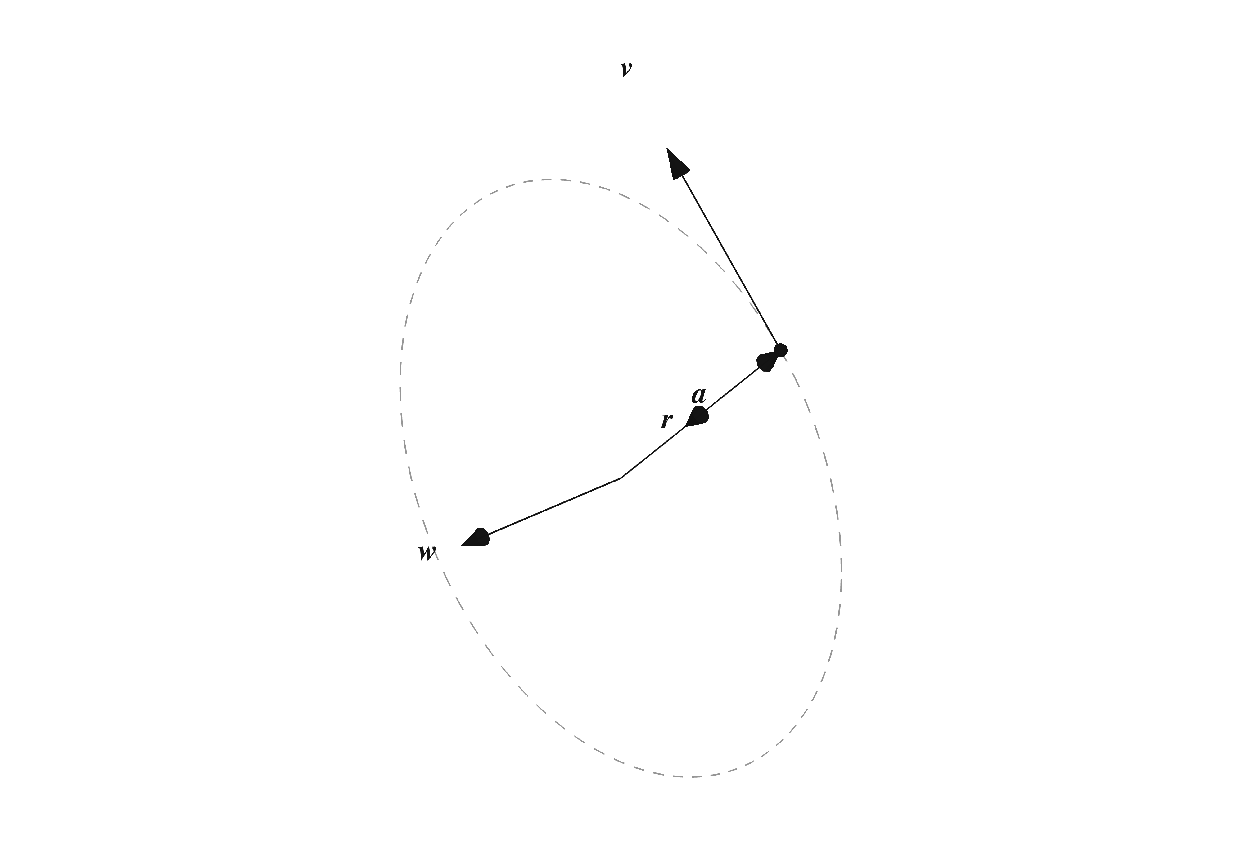
\includegraphics[width=.96\linewidth,height=.40\textheight,keepaspectratio]{figures/tecplot/concept_centripeta.pdf}
\caption[Velocidad y aceleración nominales]{Movimiento circular de un punto fijo en la base nominal del rotor. La velocidad $\vct v$ es tangente a la trayectoria y perpendicular al radio $\vct r$; la aceleración centrípeta $\vct a$ apunta hacia el eje de giro. La flecha axial indica la dirección de la velocidad angular.}\label{fig:centripeta}
\end{figure}

\subsection{Centro de masa excéntrico de una sección}
Para relacionar la cinemática con la inercia, sean $\vct a$ la posición nominal del punto de referencia de una sección respecto del cubo y $\vct c_m$ el vector que une ese punto con el centro de masa seccional. Se expresan ambos en una misma base nominal. Con traslación perturbada $\vct u$ y rotación $E$,
\begin{equation}
 \vct y_C=\vct a+\vct u+E\vct c_m,
 \qquad \vct x_C=\vct c+Q_c\vct y_C.
\end{equation}
Así,
\begin{equation}
 {}^c\vct v_C=Q_c^\tr\dot{\vct c}+W\vct y_C+\dot{\vct u}
 +\left[J_\ell(\vct\theta)\dot{\vct\theta}\right]_\times E\vct c_m,
 \label{eq:vgfull}
\end{equation}
y la velocidad angular total en componentes nominales es
\begin{equation}
 {}^c\vct\omega=\vct\Omega_c+J_\ell(\vct\theta)\dot{\vct\theta}.
\end{equation}
Si una propiedad se conoce inicialmente en la base de pala, se lleva antes a la base nominal elegida mediante su matriz de montaje. No se multiplica un tensor expresado en ejes de pala por una velocidad angular expresada en ejes de cubo sin ese cambio. Esta precaución es esencial para los efectos giroscópicos y los productos de inercia.

\section{Equilibrio de operación y movimiento síncrono}
\subsection{Estacionariedad relativa}
Una deformación constante vista desde el rotor puede seguir moviéndose respecto de $N$. Si $\vct u_c=\vct u_{c0}$ y $\vct\theta=\vct\theta_0$ son constantes, las partículas siguen trayectorias por $Q_c(t)$ aunque sus coordenadas relativas no cambien. Se habla de equilibrio relativo cuando esa configuración satisface las ecuaciones de movimiento en el sistema de referencia apropiado, no solo porque las coordenadas se mantengan constantes por definición.

La configuración de equilibrio de operación depende de velocidad, cargas y condiciones de apoyo. En ausencia de invariancia de las cargas respecto del giro, una deformación constante corrotante puede no existir. Por ejemplo, la gravedad es fija en $N$, pero sus componentes en el rotor cambian con el azimut. El cortante vertical de viento produce también una excitación periódica durante el paso de las palas.

La figura~\ref{fig:gravedad-giratoria} muestra esta diferencia con una magnitud conocida. Para la góndola horizontal y $\vct g=-g\vct E_3$, sus componentes en la base nominal del cubo son
\begin{equation}
 {}^H\vct g=({}^N\overline Q_H)^\tr(-g\vct E_3)
 =\begin{bmatrix}0\\-g\sin\psi\\-g\cos\psi\end{bmatrix}.
\end{equation}
La variación de esas componentes no significa que cambie la gravedad física. Significa que la misma dirección espacial se observa desde ejes que giran. Una operación uniforme puede, por tanto, coexistir con excitaciones periódicas en las coordenadas del rotor.

\begin{figure}[htbp]
\centering
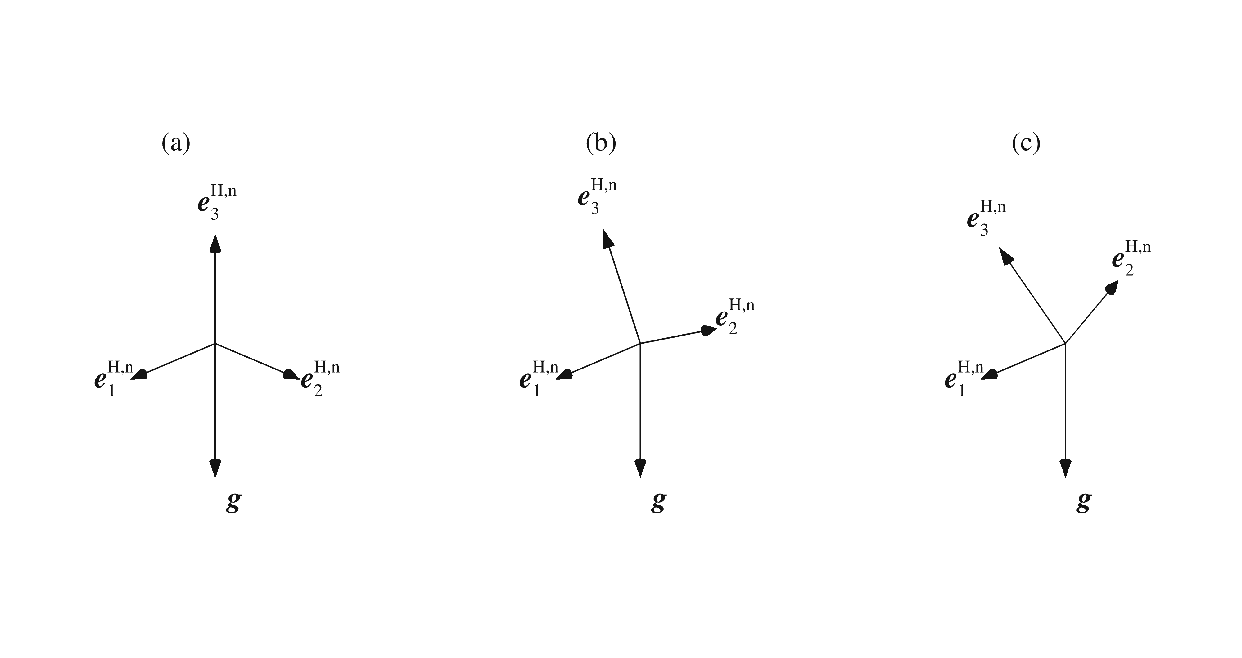
\includegraphics[width=.96\linewidth,height=.40\textheight,keepaspectratio]{figures/tecplot/concept_gravedad-giratoria.pdf}
\caption[Gravedad expresada en ejes giratorios]{La misma gravedad inercial $\vct g$ observada con tres orientaciones nominales del cubo. El vector geométrico conserva su dirección, pero sus componentes en la base $H,n$ varían con el azimut. Los paneles presentan ángulos ilustrativos.}\label{fig:gravedad-giratoria}
\end{figure}

\subsection{Estado a azimut fijo y solución periódica}
El equilibrio local calculado para un azimut $\psi_*$ no demuestra una solución periódica completa. En el primer caso se resuelve una ecuación residual algebraica con parámetros fijados; en el segundo, la trayectoria debe satisfacer las ecuaciones durante todo el período $T=2\pi/\Omega$, además de la condición de periodicidad. El término \emph{movimiento síncrono} se reserva para una respuesta ligada a la fase de giro, por ejemplo una respuesta periódica de período $T$. No toda vibración tiene que ser síncrona.

La figura~\ref{fig:operacion} ilustra la separación entre una coordenada de equilibrio constante y su perturbación vibratoria; no representa una respuesta numérica del aerogenerador.

\begin{figure}[htbp]
\centering
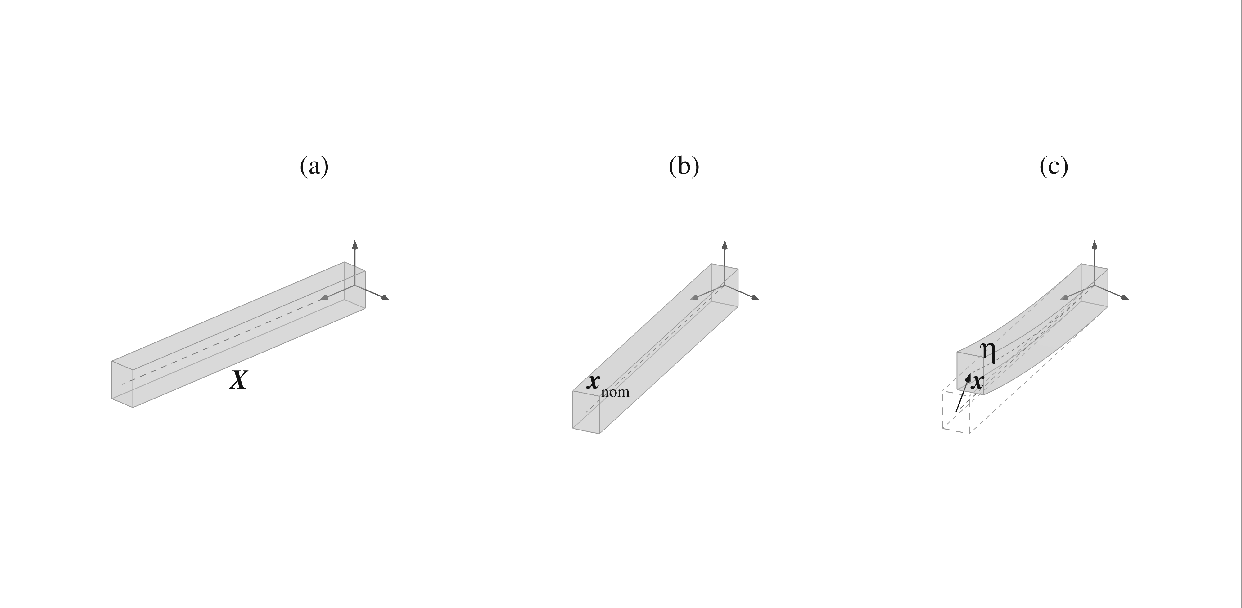
\includegraphics[width=.96\linewidth,height=.40\textheight,keepaspectratio]{figures/tecplot/concept_operacion.pdf}
\caption[Equilibrio y perturbación]{Separación geométrica entre referencia, configuración nominal y configuración actual con perturbación $\vct\eta$. El contorno discontinuo en (c) permite comparar el estado nominal con el actual. La figura ilustra una separación cinemática y no es una solución calculada de equilibrio ni una historia temporal.}\label{fig:operacion}
\end{figure}

\subsection{Vínculo con los modos de vibración}
Después de discretizar, el vector $\vct q_0$ representará las coordenadas del equilibrio, mientras $\vct\phi_j$ representará una dirección de perturbación modal. Son objetos diferentes. La relación es que las matrices linealizadas se evalúan alrededor de $\vct q_0$ y, por tanto, los modos dependen de él. No se obtiene $\vct q_0$ resolviendo el problema homogéneo de autovalores. El capítulo~\ref{ch:operacion} establece esta conexión y el caso particular en que una deformación estática admite una expansión en modos.

Las posiciones, orientaciones y velocidades definidas en este capítulo permiten calcular el movimiento de cualquier partícula de la torre, las palas y los cuerpos rígidos. Las medidas de deformación caracterizan la variación relativa entre secciones, mientras que el transporte temporal incorpora la rotación nominal. Las propiedades de masa y rigidez relacionan ahora estos campos cinemáticos con la energía cinética, la cantidad de movimiento y las fuerzas internas.
